\chapter{Dimensionamento Estrutural}
\label{dimensionamento_estrutural}

\section{Materiais de Construção}

\begin{figure}[H]
    \centering
    \begin{minipage}{1\textwidth} % Ajuste o 0.8 para aumentar ou diminuir o tamanho
        \centering
        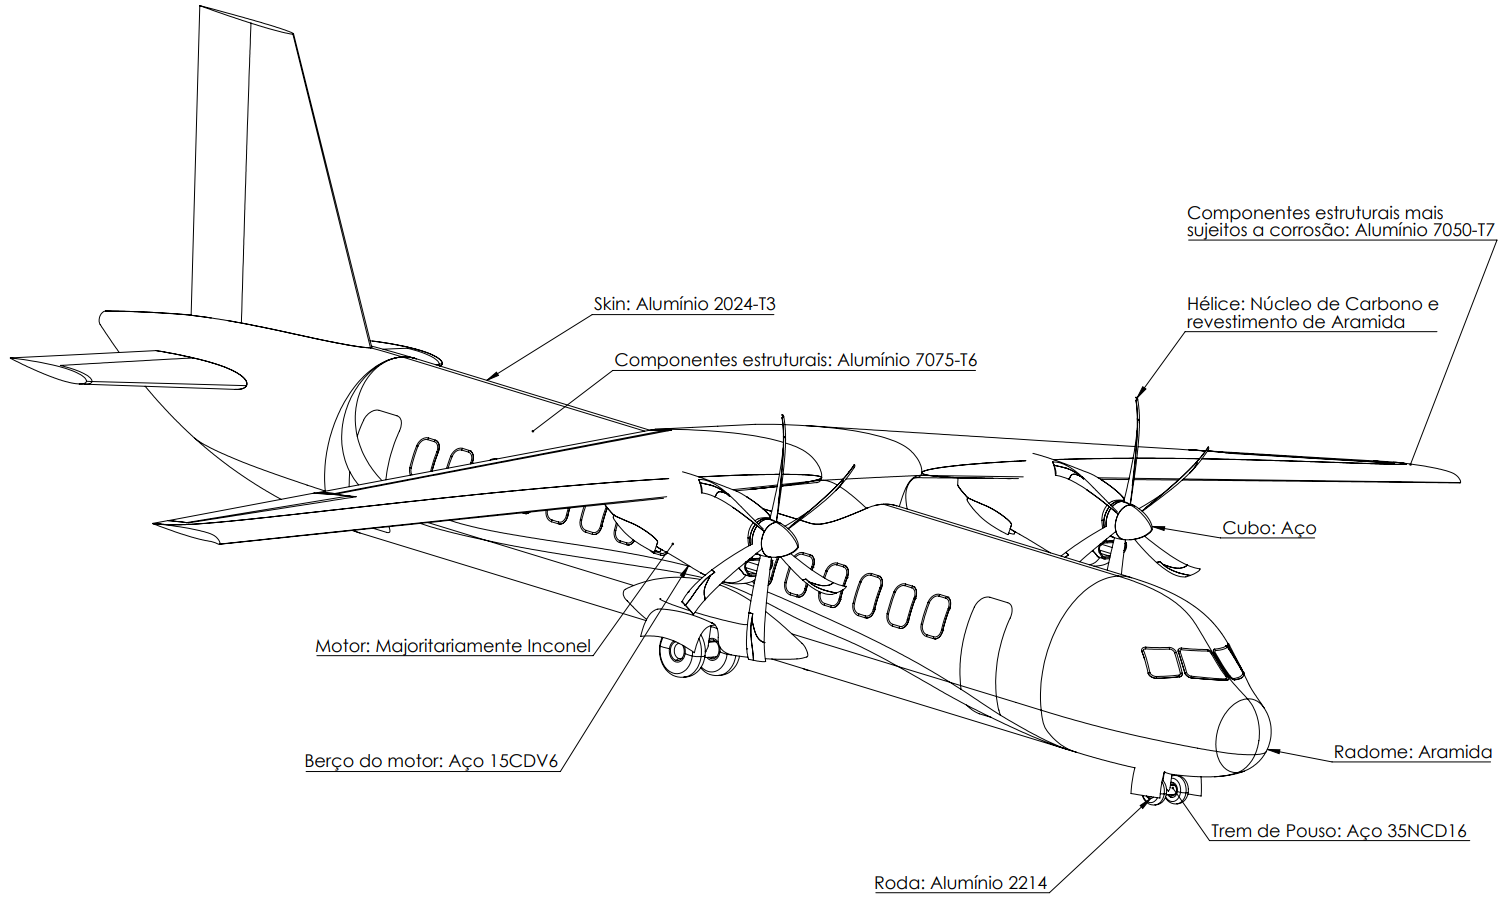
\includegraphics[width=\linewidth]{images/Materiais da aeronave.png}
        \caption{Materiais constituintes da aeronave.}
        \label{fig:Materiais da aeronave}
    \end{minipage}
\end{figure}

%Os materiais que constituem a aeronave foram escolhidos principalmente em relação às suas características serem compatíveis ao seu respectivo uso, mas houve grande inspiração nas aeronaves descritas na análise comparativa.

O radome da aeronave é fabricado em material compósito por aramida em estrutura sanduíche. Apesar de ter grande propensão ao acúmulo de água, é excelente em suportar colisões. Ademais, não interfere nas medições do radar meteorológico, posicionado logo abaixo.

Já no trem de pouso, as rodas são constituídas de uma liga de alumínio forjado 2214, com alto teor de cobre, além de ser leve, é dúctil a fim de suportar os impactos do pouso. A estrutura do trem de pouso em si é de aço 35NCD16, que tem níquel, cromo e molibdênio em sua composição, sendo altamente resistente à corrosão, já que está mais exposta, apesar do banho de proteção normalmente de cádmio; e à fadiga decorrente dos impactos durante o pouso.

No GMP, o motor PW127 é composto majoritariamente de ligas Inconel da classe 600 e 800, que são superligas de níquel. Já a hélice Hamilton Standard 568F tem pás com núcleo de carbono e revestimento de aramida, para maior resistência a danos por impacto. O cubo da hélice é de aço devido aos altos torques. Entretanto, a Hamilton não disponibiliza a liga. Por último, o berço do motor é composto por uma estrutura tubular em aço 15CDV6, pela capacidade construtiva, uma vez que apresenta excelente soldabilidade.

A célula e as superfícies sustentadoras são fabricadas em alumínio. As longarinas, nervuras, cavernas, reforçadores e longerons são de alumínio 7075-T6, que apresenta a maior resistência específica. Já em partes mais expostas, como em trilhos de fixação, será utilizada a liga 7050-T7, que apresenta melhor resistência à corrosão. O revestimento (\textit{skin}) da aeronave é composta por 2024-T3 ALCLAD, por ser mais trabalhável, podendo alcançar baixas espessuras mantendo a resistência.

A Tabela \ref{tab:propriedades_aluminio_si} sintetiza as propriedades das ligas utilizadas no dimensionamento estrutural.

\begin{table}[H]
\centering
\caption{Propriedades mecânicas das ligas de alumínio em unidades básicas do SI.}
\label{tab:propriedades_aluminio_si}
\begin{tabular}{|l|c|c|c|c|c|}
\hline
\textbf{Material} & \textbf{$E$ [GPa]} & \textbf{$\rho$ [kg/m$^3$]} & \textbf{$\nu$} & \textbf{$F_{ty}$ [MPa]} & \textbf{$F_{tu}$ [MPa]} \\ \hline
2024-T3 & $72,394$ & 2780 & 0,33 & $324,054$ & $441,264$ \\ \hline
7075-T6 & $71,016$ & 2810 & 0,33 & $503,317$ & $572,265$ \\ \hline
\end{tabular}
\end{table}

% A estrutura preliminar na fuselagem está ilustrada na imagem abaixo.

% \begin{figure}[H]
%     \centering
%     \begin{minipage}{1\textwidth} % Ajuste o 0.8 para aumentar ou diminuir o tamanho
%         \centering
%         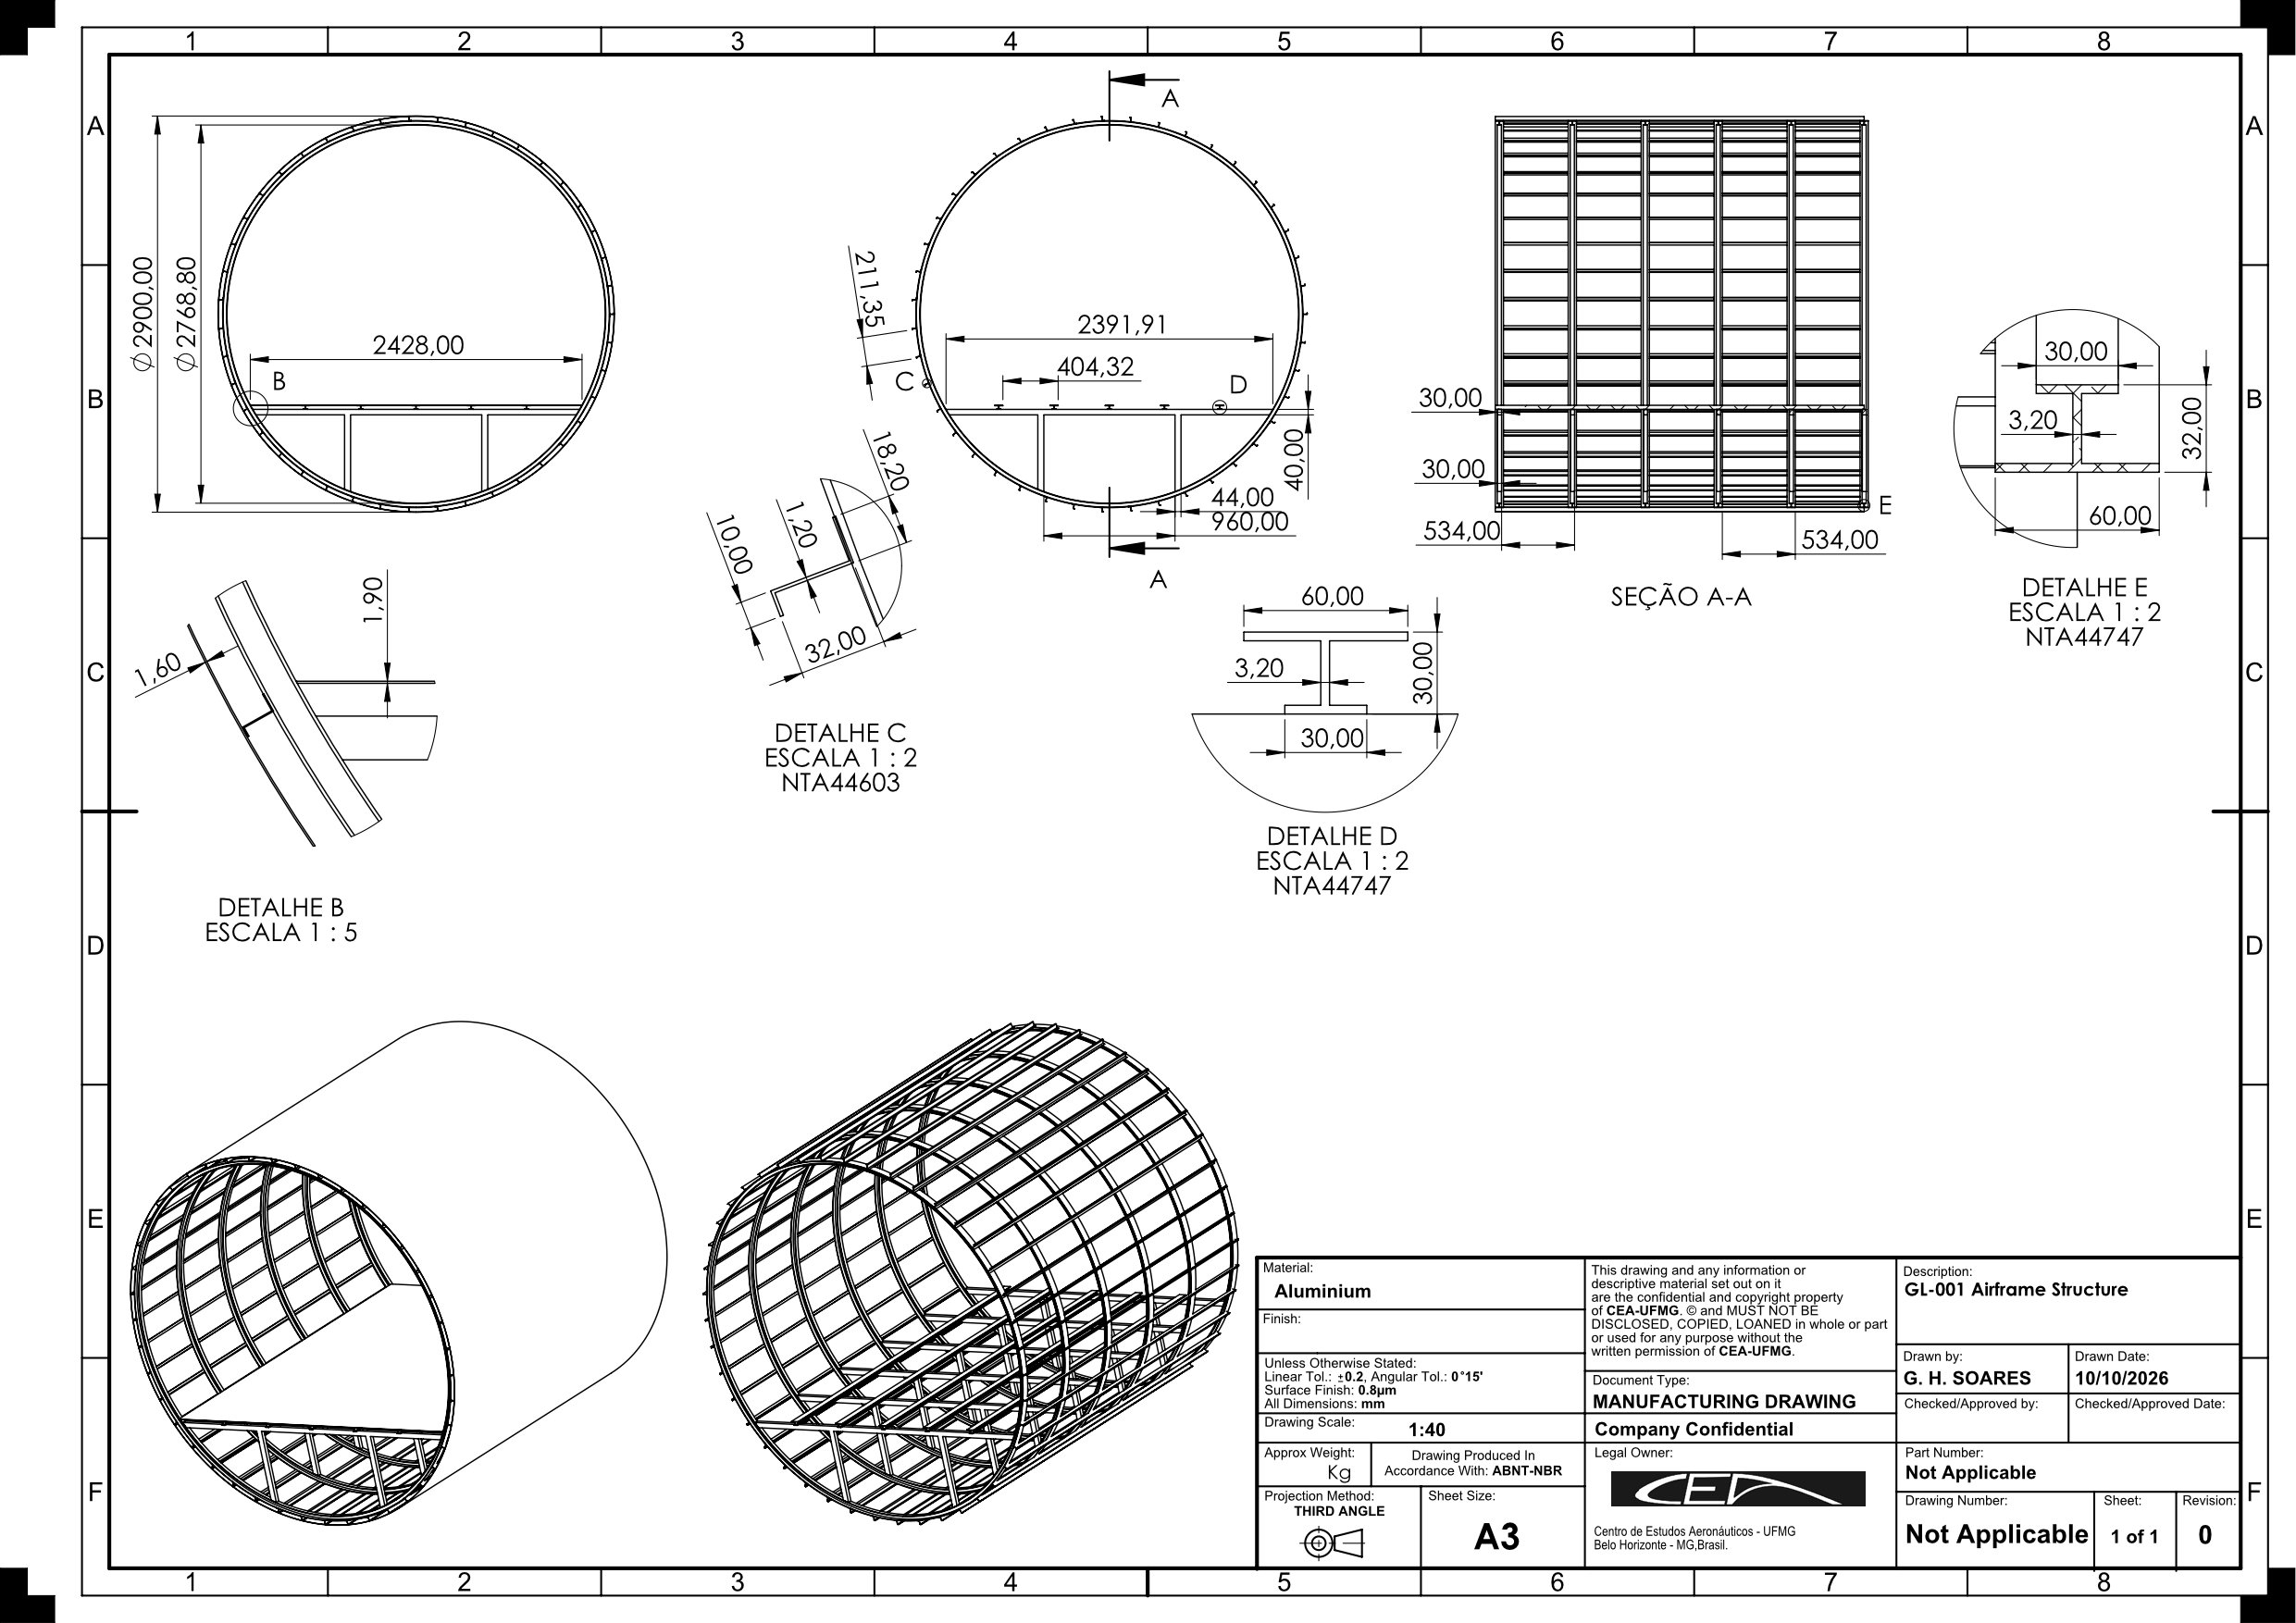
\includegraphics[width=\linewidth]{images/Estrutura interna da fuselagem2.jpg}
%         \caption{Estrutura interna da fuselagem.}
%         \label{fig:Estrutura interna da fuselagem}
%     \end{minipage}
% \end{figure}

\section{Asa}
\subsection{Longarina}
\label{sec:secao_longarina_asa}

O dimensionamento da longarina principal da asa utiliza uma seção transversal em formato I. Essa geometria apresenta eficiência estrutural para resistir aos esforços de flexão verticais, pois afasta o material da linha neutra, aumentando o momento de inércia da área. Essa distribuição de material permite a obtenção de uma estrutura com massa reduzida em comparação com seções retangulares maciças, por exemplo. 

A adoção dessa geometria estrutural mantém a consistência com as etapas prévias do projeto. Em capítulos anteriores, a seção em I já havia sido estipulada durante os cálculos preliminares associados à geometria do perfil aerodinâmico (seção 7.1.3) e à determinação da altura disponível no interior da asa. Dessa forma, o detalhamento estrutural atual parte das premissas e dos parâmetros dimensionais que foram estabelecidos ao longo do desenvolvimento aerodinâmico da aeronave.

A longarina é posicionada na coordenada de máxima espessura dos perfis aerodinâmicos ao longo de toda a envergadura. Essa localização maximiza a altura da seção transversal, resultando em um maior momento de inércia e no aumento da resistência aos esforços de flexão. Para a determinação da altura efetiva disponível para a estrutura, a espessura do revestimento externo é descontada das ordenadas do perfil aerodinâmico, permitindo a acomodação dimensional do conjunto.

O material selecionado para a longarina é a liga de alumínio 7075-T6, cujas propriedades mecânicas são compatíveis com os requisitos de projeto de elementos estruturais primários. Os parâmetros empregados no dimensionamento estão sumarizados na Tabela \ref{tab:rev_materiais}.

O dimensionamento estrutural avalia os esforços de momento fletor e de esforço cortante ao longo da envergadura. Para a asa, a análise abrange três casos de carga críticos: o caso LC4, o caso LC5 e o caso LC11.

A seção transversal em I é analisada em três pontos de interesse para a determinação do estado de tensões: a borda da mesa, a junção entre a mesa e a alma, e a linha neutra. A tensão equivalente em cada um desses pontos é avaliada com base no critério de falha de von Mises, calculado por meio da seguinte equação:

$$\sigma_{VM} = \sqrt{\sigma^2 + 3\tau^2}$$

em que $\sigma$ representa a tensão normal e $\tau$ a tensão de cisalhamento.

Os critérios de resistência adotados fundamentam-se nos requisitos do regulamento FAR/CS 25, em particular nas seções 25.303 e 25.305. A norma exige que a estrutura não apresente deformação permanente sob a aplicação das cargas limites. Desse modo, para o carregamento limite, impõe-se que a tensão equivalente não ultrapasse o limite de escoamento do material ($\sigma_{VM} \le F_{ty}$). O regulamento também estabelece que a estrutura deve ser capaz de suportar as cargas últimas sem sofrer ruptura. As cargas últimas são obtidas pela multiplicação das cargas limites por um \textbf{fator de segurança de 1,5}. Para esta condição, a tensão equivalente deve ser inferior ao limite de ruptura do material ($\sigma_{VM} \le F_{tu}$).

O parâmetro utilizado para quantificar o atendimento a esses critérios estruturais é a Margem de Segurança (MS), definida como:

$$MS = \frac{\text{tensão admissível}}{\sigma_{VM}} - 1$$

Para que o dimensionamento seja aprovado nos critérios de escoamento e de ruptura, exige-se que $MS \ge 0$.

No trecho da longarina compreendido entre a nacele e a ponta da asa, as dimensões da seção transversal são reduzidas de forma gradativa. A largura das mesas e as espessuras da alma e das mesas variam linearmente ao longo da envergadura, enquanto a altura da seção acompanha a geometria do perfil aerodinâmico local. O processo de dimensionamento avalia as margens de segurança de maneira iterativa ao longo desse segmento. Caso alguma estação apresente uma margem de segurança negativa, as espessuras estipuladas para a ponta da asa são incrementadas computacionalmente até que os requisitos de resistência sejam atendidos nas estações avaliadas.

O dimensionamento do trecho de seção constante, compreendido entre a raiz e a nacele, adotou uma largura de mesa ($b_f$) de 400 mm. A partir desse parâmetro, a altura ($H$) e as espessuras da mesa ($t_f$) e da alma ($t_w$) foram calculadas para minimizar a área da seção transversal, suportando os esforços máximos na junção com a fuselagem. As dimensões finais arredondadas da raiz podem ser consultadas nas tabelas geradas. 

\begin{table}[H]
    \centering
    \caption{Distribuição das dimensões geométricas da longarina e massa linear ao longo da semienvergadura.}
    \vspace{0.2cm}
    \begin{tabular}{cccccccc}
        \hline
        \textbf{$y$ [m]} & \textbf{Corda [m]} & \textbf{Perfil} & \textbf{$H$ [mm]} & \textbf{$b_f$ [mm]} & \textbf{$t_f$ [mm]} & \textbf{$t_w$ [mm]} & \textbf{Massa [kg/m]} \\
        \hline
        0,00 & 3,700 & NACA 43016 & 402 & 400,0 & 33,00 & 7,00 & 80,79 \\
        4,065 & 3,072 & NACA 43014 & 402 & 400,0 & 33,00 & 7,00 & 80,79 \\
        4,50 & 3,005 & NACA 43014 & 387 & 391,2 & 31,72 & 6,79 & 75,91 \\
        6,00 & 2,774 & NACA 43013 & 337 & 361,1 & 27,30 & 6,05 & 60,20 \\
        7,50 & 2,542 & NACA 43012 & 290 & 330,9 & 22,88 & 5,31 & 46,19 \\
        9,00 & 2,311 & NACA 43012 & 246 & 300,7 & 18,46 & 4,58 & 33,89 \\
        10,50 & 2,079 & NACA 43011 & 206 & 270,5 & 14,05 & 3,84 & 23,27 \\
        12,00 & 1,847 & NACA 43010 & 169 & 240,3 & 9,63 & 3,10 & 14,31 \\
        13,50 & 1,616 & NACA 43009 & 135 & 210,1 & 5,21 & 2,37 & 6,98 \\
        14,25 & 1,500 & NACA 43009 & 120 & 195,0 & 3,00 & 2,00 & 3,93 \\
        \hline
    \end{tabular}
    \label{tab:longarina_resultados_resumo}
\end{table}

Na figura \ref{fig:longarina_resumo}, são resumidas e apresentadas as dimensões da longarina ao longo da asa, bem como as margens de segurança e as folgas em algumas seções relevantes da asa.

\begin{figure}[H]
    \centering
    % Ajuste \textwidth para um tamanho menor se a imagem ficar grande demais
    % ou use \linewidth.
    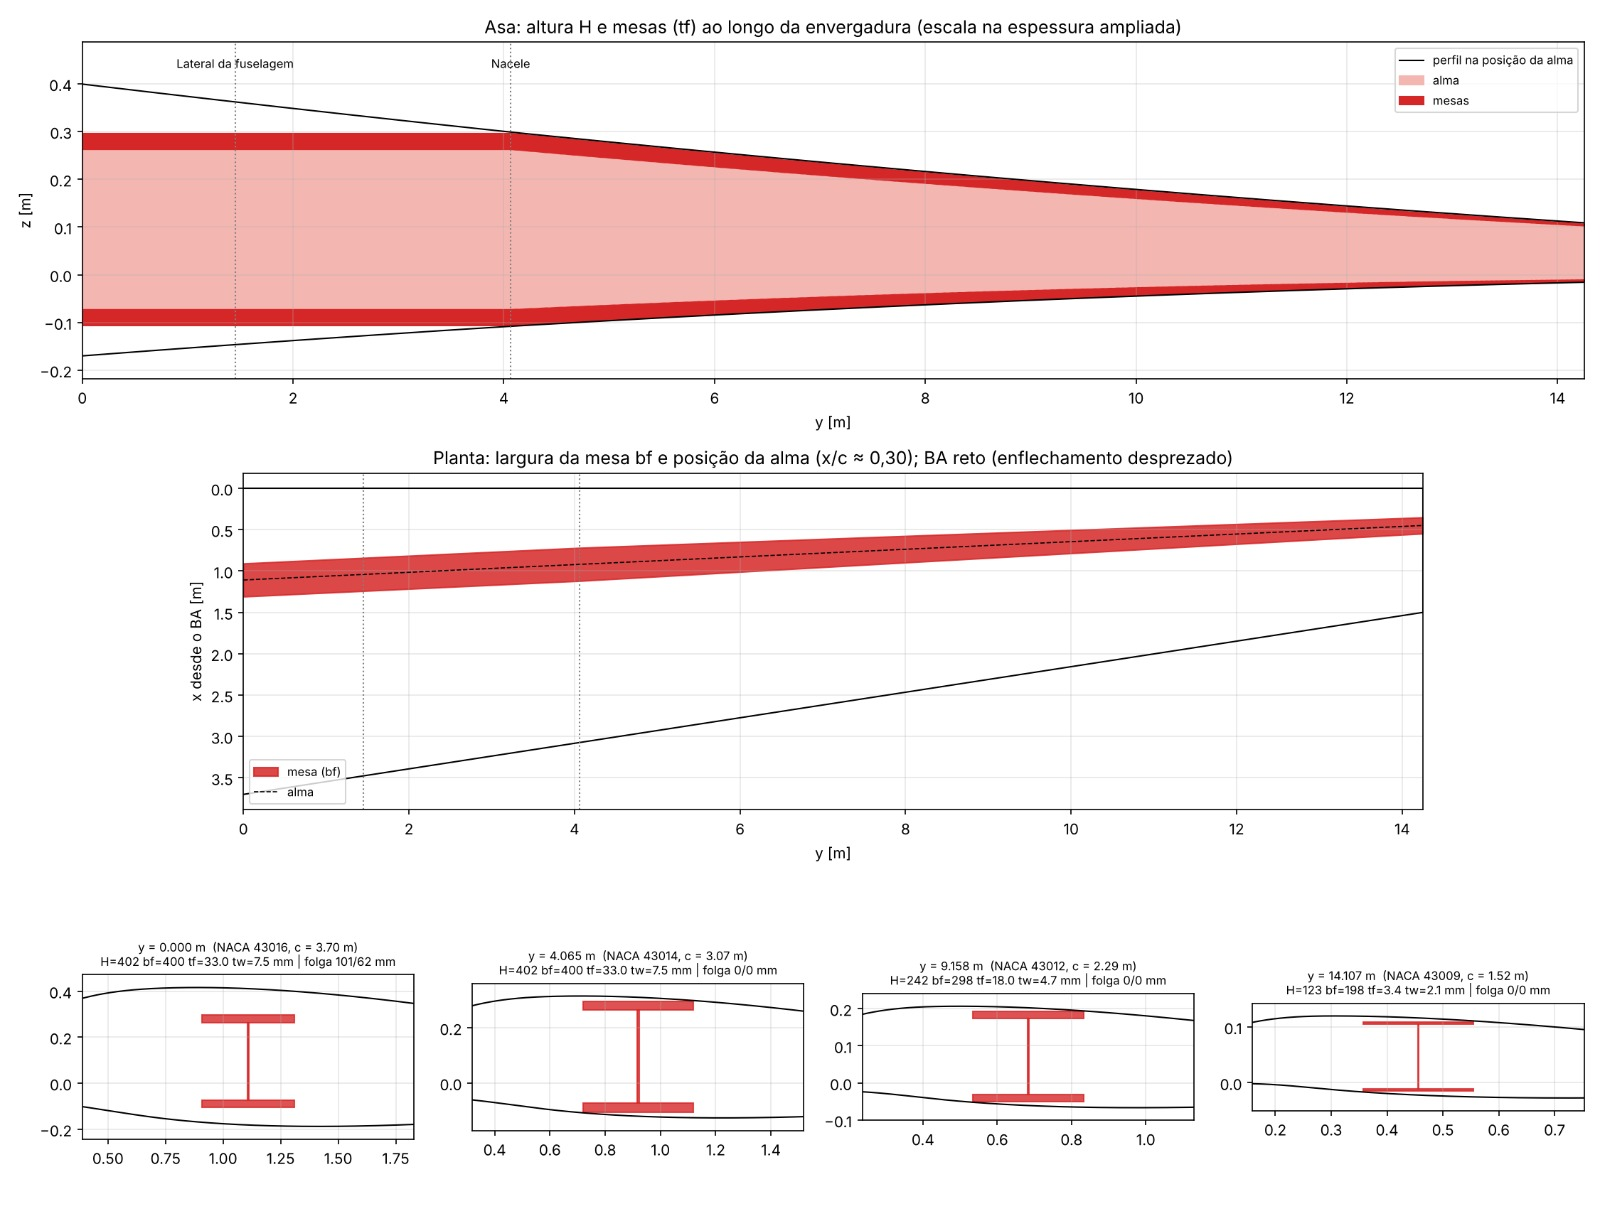
\includegraphics[width=1.0\textwidth]{parte5_longarina.jpeg}
    \caption{Resumo do dimensionamento da longarina ao longo da semienvergadura: elevação (topo), vista em planta (centro) detalhando a posição da alma ($x_{alma}$), evolução geométrica da seção transversal e margens de segurança para os casos de carga críticos (fundo).}
    \label{fig:longarina_resumo}
\end{figure}


\subsection{Nervuras}
\label{sec:nervuras}
De forma preliminar, considera-se 16 nervuras por semiasa, com espaçamento uniforme de 800\,mm a partir da ponta da asa. A seção transversal da alma é retangular, e sua altura útil é governada pela espessura relativa do perfil aerodinâmico na posição $y$ ao longo da envergadura:

\begin{equation}
    h(y) = \frac{t}{c} \cdot c(y)
    \label{eq:altura_alma}
\end{equation}

Adota-se altura efetiva da alma igual a 90\% da altura nominal, a fim de acomodar a espessura das mesas:

\begin{equation}
    h_w = 0{,}9 \cdot h(y)
\end{equation}

Para a seção de raiz, com perfil NACA\,43016 ($t/c = 0{,}16$) e corda $c_\text{raiz} = 3{,}70$\,m:

\begin{equation}
    h_w = 0{,}9 \times 0{,}16 \times 3{,}70 \approx 0{,}53\,\text{m}
\end{equation}

O critério básico de resistência ao cisalhamento impõe:

\begin{equation}
    \tau = \frac{V}{A_w} \leq \tau_\text{adm}
    \label{eq:criterio_cisalhamento}
\end{equation}

\noindent onde $A_w = h_w \cdot t_w$ é a área efetiva da alma e $\tau_\text{adm} = \tau_y / FS$ é a tensão cisalhante admissível. Adotando $\tau_y = 290$\,MPa e fator de segurança $FS = 1{,}5$, conforme requisito FAR\,25.303:

\begin{equation}
    \tau_\text{adm} = \frac{290}{1{,}5} \approx 193\,\text{MPa}
\end{equation}

A força aerodinâmica distribuída absorvida por cada nervura é obtida da derivada da distribuição de força cortante ao longo da envergadura:

\begin{equation}
    F(y) = \left(-\frac{dV}{dy}\right) \cdot \Delta y
    \label{eq:carga_nervura}
\end{equation}

\noindent onde $\Delta y = 800$\,mm é o espaçamento entre nervuras. Dimensionando para a seção de raiz ($y = 0$), região de maior carregamento:

\begin{equation}
    F(0) = 20000\,\frac{\text{N}}{\text{m}} \times 0{,}8\,\text{m}
         = 16000\,\text{N}
\end{equation}

A espessura mínima da alma resulta de:

\begin{equation}
    t_w = \frac{F(0)}{\tau_\text{adm} \cdot h_w}
        = \frac{16000}{193 \times 10^6 \times 0{,}53}
        \approx 1{,}56 \times 10^{-4}\,\text{m}
        = 0{,}156\,\text{mm}
    \label{eq:espessura_minima}
\end{equation}

\noindent Este valor é fisicamente irrealizável, pois é governado pela fabricabilidade mínima de chapas de alumínio. Adota-se, portanto, $t_w = 1{,}0$\,mm.

O resumo dos resultados obtidos estão sintetizados na Tabela \ref{tab:nervuras}, e o arranjo estrutural representado na Figura \ref{fig:cad_dimensionamento_1}.

\begin{table}[H]
\centering
\caption{Parâmetros adotados no dimensionamento preliminar das nervuras.}
\label{tab:nervuras}
\begin{tabular}{lcc}
\toprule
\textbf{Parâmetro} & \textbf{Símbolo} & \textbf{Valor} \\
\midrule
Material                          & ---              & Al\,7075-T6      \\
Nervuras por semiasa              & $n$              & 16               \\
Espaçamento                       & $\Delta y$       & 800\,mm          \\
Altura da alma (raiz)             & $h_w$            & 530\,mm          \\
Espessura mínima adotada          & $t_w$            & 1{,}0\,mm        \\
Tensão cisalhante admissível      & $\tau_\text{adm}$& 193\,MPa         \\
Fator de segurança                & $FS$             & 1{,}5            \\
Carga por nervura (raiz)          & $F(0)$           & 16000\,N      \\
\bottomrule
\end{tabular}
\end{table}

\begin{figure}[H]
    \centering
    % Ajuste o valor 0.8 para 0.7 ou 0.9 dependendo de como ficar no seu PDF
    \caption{Arranjo da longarina e das nervuras da asa.}
    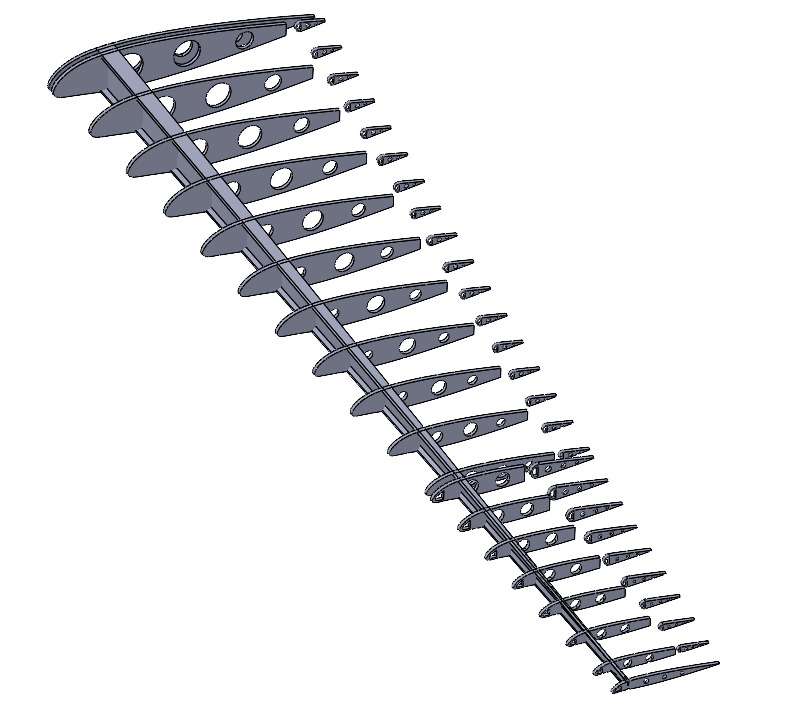
\includegraphics[width=0.6\textwidth]{Images-3-ProjetoDetalhado/cad-01.jpeg}
    \label{fig:cad_dimensionamento_1}
\end{figure}

\subsection{Revestimento}

O revestimento da asa, formado pelo painel e pelos reforçadores longitudinais, foi dimensionado pelo método de Megson \cite{megson2007}. Cada vão entre nervuras é analisado na sua seção interna, que é a mais carregada, e recebe a menor espessura de painel que mantém margem de segurança $MS \ge 0$ em todos os critérios de falha, sob carga última. Os vãos são delimitados pelas nervuras da Seção~\ref{sec:nervuras}, espaçadas de 800\,mm. O primeiro vão vai da lateral da fuselagem ($y = 1{,}45$\,m) até a primeira nervura ($y = 2{,}25$\,m), o que resulta em 16 vãos de 800\,mm por semiasa. A longarina principal é a definida na Seção~\ref{sec:secao_longarina_asa} e faz parte da mesma seção resistente.
 
\subsubsection{Considerações}
 
\begin{itemize}
    \item O diedro e o enflechamento foram desprezados: a linha de 25\% da corda é tomada como reta;
    \item Célula de torção única, em D: o revestimento vai do bordo de ataque até a longarina principal, a 30\% da corda (máxima espessura do perfil), e é fechado pela alma da longarina. O revestimento atrás da longarina é tratado como carenagem e não faz parte da seção resistente;
    \item A longarina principal tem as dimensões $H$, $b_f$, $t_f$ e $t_w$ da Tabela~\ref{tab:longarina_resultados_resumo}, interpoladas linearmente em $y$, e fica centrada na altura local do perfil. A flexão é dividida entre o revestimento e as mesas da longarina, na proporção da rigidez de cada um. A alma da longarina é estendida até o painel para fechar a célula;
    \item A alma da longarina resiste apenas ao cisalhamento;
    \item As cargas foram multiplicadas pelo fator de segurança de 1,5 (\S~25.303 do 14 CFR Part 25). As cargas são apenas aerodinâmicas, sem alívio de inércia do peso da asa, do combustível e do motor;
    \item Painel com reforçadores em Z de espessura igual à do painel ($t_{st} = t_{sk}$), com espaçamento máximo $b_s = 120$\,mm, alma de altura $h_{st} = 60$\,mm e flanges de largura $f_{st} = 0{,}30\,h_{st}$ (Figura~\ref{fig:rev_reforcador});
    \item Espessuras de painéis consideradas: 1,6; 2,0; 2,5; 3,0; 3,5; 4,0; 4,5; 5,0; 5,5; 6,0; 6,5; 7,0; 8,0; 9,0; 10,0; 11,0 e 12,0\,mm;
    \item Propriedades mecânicas conforme seção \ref{tab:propriedades_aluminio_si}.
\end{itemize}

\begin{figure}[H]
    \centering
    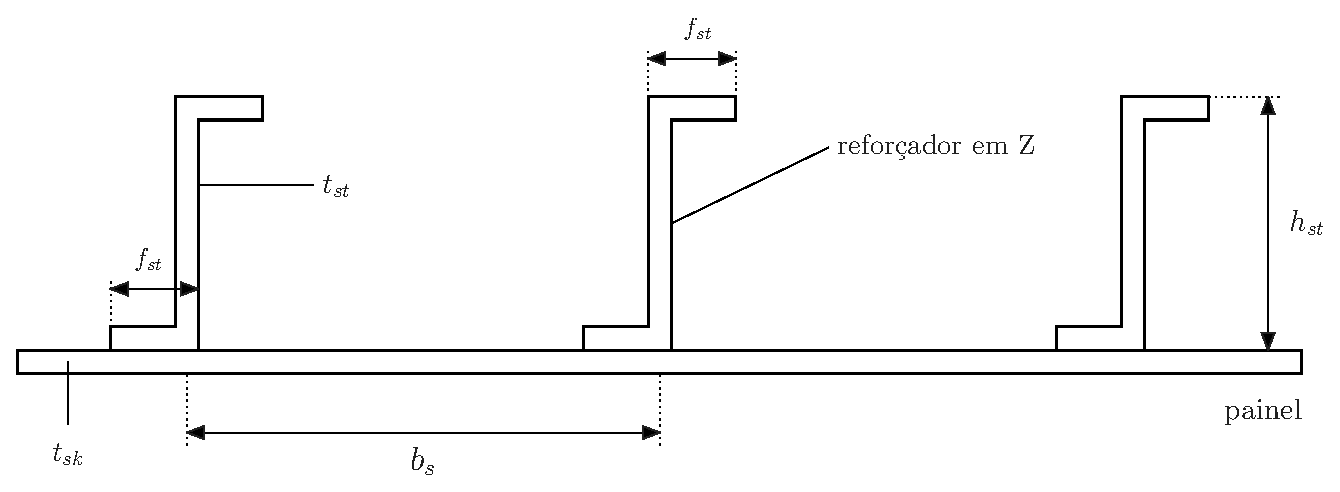
\includegraphics[width=0.9\linewidth]{images/esquema_reforcador.eps}
    \caption{Esquema do painel com reforçadores em Z: altura da alma $h_{st}$, largura das abas $f_{st}$, espessura do reforçador $t_{st}$, espessura do painel $t_{sk}$ e passo $b_s$.}
    \label{fig:rev_reforcador}
\end{figure}
 
\subsubsection{Materiais}
 
Os dois revestimentos trabalham de forma diferente e receberam ligas diferentes (Tabela~\ref{tab:rev_materiais}). O extradorso fica comprimido nas condições de fator de carga positivo, e o que o limita é a flambagem e o escoamento em compressão. Por isso, adotou-se a liga Al\,7075-T6, cuja tensão de escoamento em compressão é 72\% maior que a da liga Al\,2024-T3. O intradorso é tracionado a cada voo, e sua vida é limitada pela fadiga e pela propagação de trincas, que crescem apenas sob tração. Por isso, adotou-se a liga Al\,2024-T3, que tem menor resistência estática, mas maior tenacidade e menor taxa de propagação de trinca. Os reforçadores são de Al\,7075-T6 extrudado.
 
\begin{table}[H]
\centering
\caption{Propriedades dos materiais do revestimento (base A do MIL-HDBK-5, conforme Niu \cite{niu1999})}
\label{tab:rev_materiais}
\small
\begin{tabular}{lccc}
\toprule
 & \makecell{\textbf{Painel do}\\\textbf{extradorso}} & \makecell{\textbf{Painel do}\\\textbf{intradorso}} & \textbf{Reforçadores} \\
\midrule
Liga                                                    & Al\,7075-T6 & Al\,2024-T3 & Al\,7075-T6 \\
Forma                                                   & chapa       & chapa       & extrudado   \\
Escoamento em compressão, $F_{cy}$ [MPa]                & 462         & 269         & 483         \\
Escoamento em tração, $F_{ty}$ [MPa]                    & 476         & 324         & 483         \\
Resistência à tração, $F_{tu}$ [MPa]                    & 524         & 441         & 538         \\
Resistência ao cisalhamento, $F_{su}$ [MPa]             & 296         & 269         & 290         \\
\bottomrule
\end{tabular}
\end{table}
 
\subsubsection{Dados da seção da raiz}
 
As contas a seguir são da seção $y = 1{,}45$\,m, na lateral da fuselagem. Os demais vãos seguem a mesma sequência, e os resultados estão apresentados nas Tabelas~\ref{tab:rev_extradorso} a~\ref{tab:rev_torcao}. A corda local e a espessura relativa são:
 
\begin{equation}
    c(y) = c_{raiz} - (c_{raiz} - c_{ponta})\,\frac{y}{b/2} = 3{,}70 - 2{,}20 \cdot \frac{1{,}45}{14{,}25} = 3{,}476\,\text{m}
    \label{eq:rev_corda}
\end{equation}
 
\begin{equation}
    \frac{t}{c} = 0{,}16 - 0{,}07 \cdot \frac{1{,}45}{14{,}25} = 0{,}153
    \label{eq:rev_tc}
\end{equation}
 
O contorno da célula segue o perfil NACA\,430xx com a espessura relativa da Equação~\ref{eq:rev_tc}, discretizado em 400 pontos por revestimento. A origem fica no eixo de referência das cargas (25\% da corda, sobre a linha da corda), com $x$ para trás, $y$ ao longo da envergadura e $z$ para cima. Na raiz:
 
\begin{itemize}
    \item altura da célula na longarina: $402$\,mm; o bordo de ataque fica $869{,}0$\,mm à frente do eixo de referência;
    \item perímetro do revestimento entre o bordo de ataque e a longarina: $1228{,}4$\,mm no extradorso e $1065{,}7$\,mm no intradorso, o que comporta $n_{st} = 10$ reforçadores no extradorso e $8$ no intradorso, com espaçamentos de $111{,}7$\,mm e $118{,}4$\,mm;
    \item área interna da célula:
    \begin{equation}
        2A_c = \sum_{j} \left(z_j\,x_{j+1} - x_j\,z_{j+1}\right) = 9{,}0553 \times 10^{5}\,\text{mm}^2 \quad\Rightarrow\quad A_c = 452767\,\text{mm}^2
        \label{eq:rev_area}
    \end{equation}
    \item comprimento do vão $\Delta y = 800$\,mm; alma do reforçador $h_{st} = 60$\,mm e flanges $f_{st} = 18$\,mm.
\end{itemize}
 
 
\begin{table}[H]
\centering
\caption{Cargas últimas na seção da raiz ($y = 1{,}45$\,m).}
\label{tab:rev_cargas_raiz}
\begin{tabular}{lccccc}
\toprule
\textbf{Caso} & \makecell{\boldmath$S_z$\\\textbf{[kN]}} & \makecell{\boldmath$M_x$\\\textbf{[kN$\cdot$m]}} & \makecell{\boldmath$M_y$\\\textbf{[kN$\cdot$m]}} & \makecell{\boldmath$S_x$\\\textbf{[kN]}} & \makecell{\boldmath$M_z$\\\textbf{[kN$\cdot$m]}} \\
\midrule
LC4 (manobra, $V_D$, $n_z = 2{,}5$) & $438{,}7$ & $2396$ & $-310{,}4$ & $-19{,}3$ & $104{,}7$ \\
LC5 (manobra, $V_{S,\mathrm{neg}}$, $n_z = -1{,}0$) & $-149{,}6$ & $-817$ & $-66{,}2$ & $-34{,}8$ & $189{,}8$ \\
LC11 (rajada positiva, $V_D$) & $330{,}6$ & $1805$ & $-310{,}4$ & $-4{,}3$ & $23{,}0$ \\
\bottomrule
\end{tabular}
\end{table}
 
\noindent Na Tabela~\ref{tab:rev_cargas_raiz}, $S_z$ é o esforço cortante vertical, $M_x$ o momento fletor, $M_y$ o momento torsor em torno do eixo de referência, $S_x$ o esforço cortante no plano da corda e $M_z$ o momento fletor nesse plano.
 
\subsubsection{Seção idealizada}
 
A seção é idealizada com um \textit{boom} em cada reforçador, um em cada canto da célula (junto à longarina e no bordo de ataque, de cada lado) e um em cada mesa da longarina principal. Cada \textit{boom} de reforçador concentra a área do reforçador e a metade de cada painel vizinho. Nos cantos, o \textit{boom} recebe apenas a metade do painel vizinho. Cada mesa da longarina é um \textit{boom} de área $b_f t_f$, posicionado no centroide da mesa. Os painéis entre \textit{booms} e a alma da longarina resistem apenas a cisalhamento. Para o extradorso da raiz, com painel de $5{,}0$\,mm e espaçamento $b_s = 111{,}7$\,mm, os elementos estão na Tabela~\ref{tab:rev_booms}. A \autoref{fig:rev_secao_celula_D} ilustra a seção idealizada.
 
\begin{table}[H]
\centering
\caption{Composição dos \textit{booms} do extradorso na raiz.}
\label{tab:rev_booms}
\begin{tabular}{lc}
\toprule
\textbf{Elemento} & \textbf{Área [mm$^2$]} \\
\midrule
Aba ligada ao painel $18 \times 5{,}0$                  & $90$ \\
Alma $60 \times 5{,}0$                                 & $300$ \\
Aba livre $18 \times 5{,}0$                            & $90$ \\
\midrule
Reforçador, $A_{st}$                                    & $480$ \\
Painel, $b_s \times t_{sk} = 111{,}7 \times 5{,}0$      & $558{,}4$ \\
\midrule
\textit{Boom} de reforçador, $B_{st} = A_{st} + b_s t_{sk}$     & $1038{,}4$ \\
\textit{Boom} de canto, $B_{c} = b_s t_{sk}/2$                  & $279{,}2$ \\
\textit{Boom} da mesa da longarina, $b_f t_f = 400 \times 33$ & $13200$ \\
\bottomrule
\end{tabular}
\end{table}
 
\noindent Para o intradorso, com painel de $7{,}0$\,mm e espaçamento de $118{,}4$\,mm: $A_{st} = 672$\,mm$^2$, $B_{st} = 1500{,}9$\,mm$^2$ e $B_c = 414{,}4$\,mm$^2$. A seção da raiz tem, portanto, $24$ \textit{booms} ($10$ reforçadores e 2 cantos no extradorso, $8$ reforçadores e 2 cantos no intradorso e as 2 mesas da longarina), ligados por $20$ painéis e pela alma da longarina.
 
\noindent A espessura equivalente, $t_{eq} = \sum B / s$, é a de uma chapa com a mesma área dos \textit{booms} de um revestimento de perímetro $s$, sem as mesas da longarina: na raiz, $8{,}91$\,mm no extradorso e $12{,}04$\,mm no intradorso. Ela é usada apenas para apresentar os resultados e calcular a massa.

\begin{figure}[H]
    \centering
    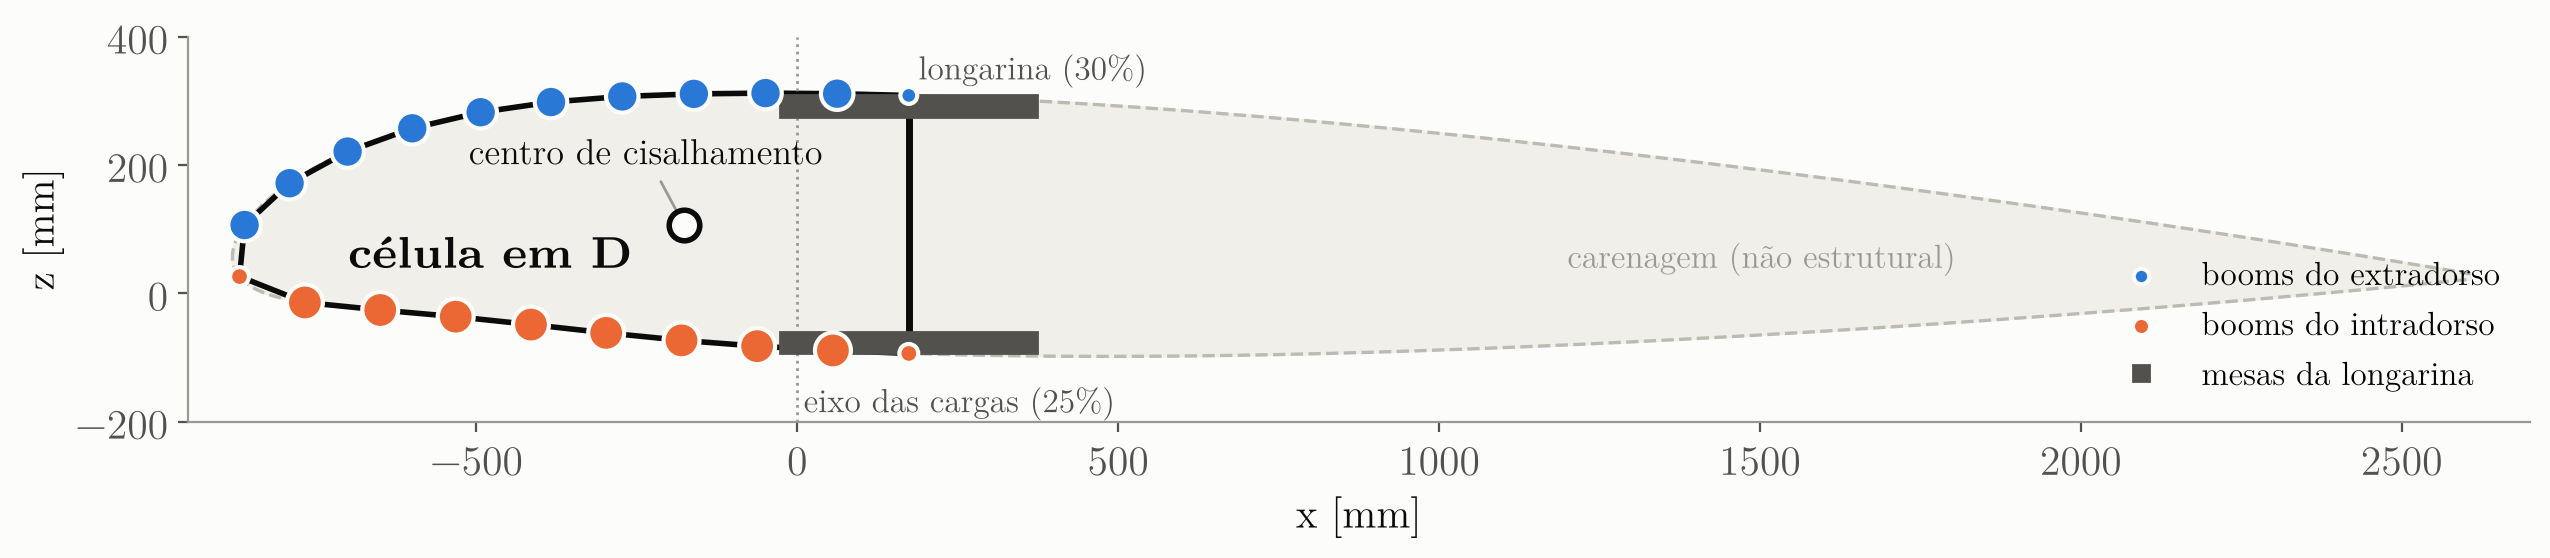
\includegraphics[width=1\linewidth]{1_secao_celula_D.png}
    \caption{Esquema da seção resistente da asa na raiz: célula em D, formada pelo painel do bordo de ataque e pela alma da longarina principal.}
    \label{fig:rev_secao_celula_D}
\end{figure}
 
\subsubsection{Tensão normal}
 
A tensão normal de flexão pode ser definida por:
 
\begin{equation}
    \sigma = a_x\,x + a_z\,z, \qquad
    a_x = \frac{M_z I_{xx} + M_x I_{xz}}{D}, \qquad
    a_z = -\frac{M_x I_{zz} + M_z I_{xz}}{D}
    \label{eq:rev_sigma}
\end{equation}

sendo,

\begin{equation}
    D = I_{xx} I_{zz} - I_{xz}^2 = 1{,}2254 \times 10^{19}\,\text{mm}^8
    \label{eq:rev_D}
\end{equation}
 
Para o caso LC4, com $M_x = 2{,}396 \times 10^{9}$\,N$\cdot$mm e $M_z = 1{,}047 \times 10^{8}$\,N$\cdot$mm, resultam $a_x = 0{,}05042$\,MPa/mm e $a_z = -1{,}2011$\,MPa/mm. No ponto mais comprimido do extradorso ($x = -69{,}8$\,mm e $z = 281{,}3$\,mm, em relação ao centroide):
 
\begin{equation}
    \sigma = -3{,}5 + (-337{,}9) = -341{,}4\,\text{MPa}
    \label{eq:rev_sigma_max}
\end{equation}
 
A Tabela~\ref{tab:rev_tensoes_raiz} resume as tensões máximas dos três casos.
 
\begin{table}[H]
\centering
\caption{Tensões normais últimas na raiz.}
\label{tab:rev_tensoes_raiz}
\begin{tabular}{lcccc}
\toprule
\textbf{Caso} & \makecell{\textbf{Extradorso}\\\textbf{[MPa]}} & \makecell{\textbf{Intradorso}\\\textbf{[MPa]}} & \makecell{\textbf{Mesa superior}\\\textbf{[MPa]}} & \makecell{\textbf{Mesa inferior}\\\textbf{[MPa]}} \\
\midrule
LC4 & $-341{,}4$ & $318{,}4$ & $-222{,}8$ & $220{,}4$ \\
LC5 & $118{,}3$ & $-98{,}0$ & $85{,}1$ & $-64{,}9$ \\
LC11 & $-256{,}4$ & $237{,}3$ & $-170{,}1$ & $163{,}6$ \\
\bottomrule
\end{tabular}
\end{table}
 
\subsubsection{Fluxo de cisalhamento}
 
Como a asa afila ao longo da envergadura, os \textit{booms} são inclinados, e a componente vertical da sua carga resiste a parte do cortante. Para o caso LC4, somando extradorso, intradorso e mesas da longarina:
 
\begin{equation}
    P_z = \sigma B \frac{\mathrm{d}z}{\mathrm{d}y}, \qquad
    \sum P_z = 63{,}1 + 35{,}2 + 0{,}2 = 98{,}5\,\text{kN}
    \label{eq:rev_Pz}
\end{equation}
 
\begin{equation}
    \begin{gathered}
        S_{z,w} = S_z - \sum P_z = 438{,}7 - 98{,}5 = 340{,}2\,\text{kN} \\
        S_{x,w} = S_x - \sum P_x = -19{,}25 - (-9{,}64) = -9{,}61\,\text{kN}
    \end{gathered}
    \label{eq:rev_Sw}
\end{equation}
 
A seção é cortada no primeiro painel do extradorso, e o fluxo da seção aberta é acumulado \textit{boom} a \textit{boom}, assim, conforme Megson:
 
\begin{equation}
    q_{b,r} = q_{b,r-1} - \left[\frac{S_{x,w} I_{xx} - S_{z,w} I_{xz}}{D}\, x_r + \frac{S_{z,w} I_{zz} - S_{x,w} I_{xz}}{D}\, z_r\right] B_r
    \label{eq:rev_qb}
\end{equation}
 
O fluxo constante que fecha a seção vem do equilíbrio de momentos em torno do eixo de referência das cargas (Eq.~(17.17) do Megson), em que $p$ é o braço de cada painel em relação a esse eixo e $\sum p\,\mathrm{d}s = 2A_c$:
 
\begin{equation}
    \begin{aligned}
        q_{s,0} &= \frac{M_y - \sum (z P_x - x P_z) - \sum q_b\, p\, \mathrm{d}s}{2A_c} \\
        &= \frac{\left[-310{,}4 + (-15{,}2) + 176{,}3\right] \times 10^{6}}{0{,}9055 \times 10^{6}} = -164{,}8\,\text{N/mm}
    \end{aligned}
    \label{eq:rev_qs0}
\end{equation}
 
O fluxo total é $q = q_b + q_{s,0}$. No extradorso, ele varia de $-165$\,N/mm junto ao bordo de ataque a $-560$\,N/mm junto à longarina. Na alma da longarina, entre as mesas, o fluxo é $-993{,}4$\,N/mm: como as mesas são \textit{booms} de grande área, é nesse trecho que a longarina leva a maior parte do cortante vertical. As tensões de cisalhamento máximas são:
 
\begin{equation}
    \begin{gathered}
        \tau_{extr} = \frac{560{,}3}{5{,}0} = 112{,}1\,\text{MPa}, \qquad
        \tau_{intr} = \frac{564{,}8}{7{,}0} = 80{,}7\,\text{MPa} \\
        \tau_{w} = \frac{993{,}4}{7{,}0} = 141{,}9\,\text{MPa}
    \end{gathered}
    \label{eq:rev_tau}
\end{equation}
 
\noindent em que $\tau_w$ é a tensão na alma da longarina.
 
\begin{table}[H]
\centering
\caption{Cisalhamento último na seção da raiz.}
\label{tab:rev_cisalhamento_raiz}
\begin{tabular}{lccccc}
\toprule
\textbf{Caso} & \makecell{\boldmath$S_{z,w}$\\\textbf{[kN]}} & \makecell{\boldmath$q_{s,0}$\\\textbf{[N/mm]}} & \makecell{\boldmath$\tau_{extr}$\\\textbf{[MPa]}} & \makecell{\boldmath$\tau_{intr}$\\\textbf{[MPa]}} & \makecell{\boldmath$\tau_{w}$\\\textbf{[MPa]}} \\
\midrule
LC4 & $340{,}2$ & $-164{,}8$ & $112{,}1$ & $80{,}7$ & $141{,}9$ \\
LC5 & $-115{,}9$ & $-128{,}5$ & $26{,}0$ & $17{,}6$ & $21{,}8$ \\
LC11 & $256{,}3$ & $-210{,}0$ & $100{,}7$ & $73{,}7$ & $119{,}1$ \\
\bottomrule
\end{tabular}
\end{table}
 
\subsubsection{Centro de cisalhamento e torção}
 
O equilíbrio de momentos da Equação~\ref{eq:rev_qs0} resolve cortante e torção em conjunto. Para separar as duas parcelas, calcula-se o centro de cisalhamento (CC), transfere-se a carga para ele e trata-se o momento resultante como torção pura. Nesta parte, a correção de afilamento não é aplicada. As paredes que resistem ao cisalhamento são os painéis e a alma da longarina:
 
\begin{equation}
    \oint \frac{\mathrm{d}s}{t} = \frac{1228{,}4}{5{,}0} + \frac{1065{,}7}{7{,}0} + \frac{402}{7{,}0} = 245{,}7 + 152{,}2 + 76{,}0 = 473{,}9
    \label{eq:rev_dst}
\end{equation}
 
Aplicando uma força unitária $S_z = 1$\,N, calcula-se o fluxo da seção aberta pela Equação~\ref{eq:rev_qb} e fecha-se a seção pela condição de giro nulo (Eq.~(17.27) do Megson):
 
\begin{equation}
    q_{s,0} = -\frac{\oint (q_b/t)\,\mathrm{d}s}{\oint \mathrm{d}s/t} = -\frac{-0{,}3569}{473{,}9} = 7{,}530 \times 10^{-4}\,\text{N/mm por N}
    \label{eq:rev_qs0_cc}
\end{equation}
 
O momento desse fluxo em torno do eixo de referência é igual ao da força aplicada no centro de cisalhamento, $-x_{cc} S_z$:
 
\begin{equation}
    \begin{aligned}
        \sum q\,p\,\mathrm{d}s &= \sum q_b\,p\,\mathrm{d}s + q_{s,0}\,(2A_c) \\
        &= -513{,}9 + \left(7{,}530 \times 10^{-4}\right)\left(9{,}0553 \times 10^{5}\right) = 167{,}9\,\text{N}\cdot\text{mm}
    \end{aligned}
    \label{eq:rev_xcc}
\end{equation}
 
Portanto, $x_{cc} = -167{,}9$\,mm: o centro de cisalhamento fica $167{,}9$\,mm à frente do eixo de referência, ou seja, a $0{,}25 - 167{,}9/3476 = 0{,}202$ da corda ($20{,}2$\%). Repetindo o cálculo com $S_x = 1$\,N, obtém-se $\sum q_b\,p\,\mathrm{d}s = 152{,}6$\,N$\cdot$mm e $q_{s,0} = -7{,}886 \times 10^{-5}$\,N/mm, de onde $z_{cc} = 81{,}2$\,mm acima da linha da corda. O momento torsor em torno do centro de cisalhamento é:
 
\begin{equation}
    T = M_y + x_{cc} S_z - z_{cc} S_x
    \label{eq:rev_T}
\end{equation}
 
\noindent O primeiro termo é o momento de arfagem das cargas; o segundo vem da sustentação, que atua cerca de $5$\% da corda atrás do centro de cisalhamento e, por isso, também tende a baixar o nariz; o terceiro vem da força no plano da corda (Tabela~\ref{tab:rev_torque_raiz}).
 
\begin{table}[H]
\centering
\caption{Momento torsor último em torno do centro de cisalhamento, na raiz.}
\label{tab:rev_torque_raiz}
\begin{tabular}{lcccc}
\toprule
\textbf{Caso} & \makecell{\boldmath$M_y$\\\textbf{[kN$\cdot$m]}} & \makecell{\boldmath$x_{cc} S_z$\\\textbf{[kN$\cdot$m]}} & \makecell{\boldmath$-z_{cc} S_x$\\\textbf{[kN$\cdot$m]}} & \makecell{\boldmath$T$\\\textbf{[kN$\cdot$m]}} \\
\midrule
LC4 & $-310{,}4$ & $-73{,}7$ & $1{,}6$ & $-382{,}5$ \\
LC5 & $-66{,}2$ & $25{,}1$ & $2{,}8$ & $-38{,}3$ \\
LC11 & $-310{,}4$ & $-55{,}5$ & $0{,}4$ & $-365{,}5$ \\
\bottomrule
\end{tabular}
\end{table}
 
O caso crítico em torção é o LC4: com o centro de cisalhamento à frente do eixo das cargas, a sustentação soma-se ao momento de arfagem, e o LC4 é o caso de maior sustentação. O fluxo de torção pura, segundo Megson, é definido por:
 
\begin{equation}
    q_T = \frac{T}{2A_c} = \frac{-382{,}5 \times 10^{6}}{9{,}0553 \times 10^{5}} = -422{,}4\,\text{N/mm}
    \label{eq:rev_qT}
\end{equation}
 
\noindent o que corresponde a $84{,}5$\,MPa no painel do extradorso, $60{,}3$\,MPa no do intradorso, $60{,}3$\,MPa na alma da longarina. A rigidez torcional da célula é:
 
\begin{equation}
    J = \frac{(2A_c)^2}{\oint \mathrm{d}s/t} = 1{,}730 \times 10^{9}\,\text{mm}^4, \qquad GJ = 4{,}671 \times 10^{13}\,\text{N}\cdot\text{mm}^2 = 46{,}7\,\text{MN}\cdot\text{m}^2
    \label{eq:rev_J}
\end{equation}
 
A taxa de giro é calculada com o momento torsor limite, igual ao último dividido por 1,5. Para o caso LC4, na raiz:
 
\begin{equation}
    \frac{\mathrm{d}\theta}{\mathrm{d}y} = \frac{T/1{,}5}{GJ} = \frac{-255{,}0 \times 10^{6}}{4{,}671 \times 10^{13}} = -5{,}458 \times 10^{-6}\,\text{rad/mm} = -0{,}3127\,^\circ\text{/m}
    \label{eq:rev_dtheta}
\end{equation}
 
O giro é integrado a partir da nervura da raiz, considerada engastada, com momento torsor nulo na ponta:
 
\begin{equation}
    \theta_{i+1} = \theta_i + \frac{1}{2}\left(\theta'_i + \theta'_{i+1}\right) \Delta y_i
    \label{eq:rev_theta}
\end{equation}
 
\noindent No primeiro vão, $\theta_2 = \tfrac{1}{2}\left[-0{,}3127 + (-0{,}3598)\right] \times 0{,}8 = -0{,}269^\circ$. Os demais vãos estão na Tabela~\ref{tab:rev_torcao}.
 
\subsubsection{Resultados por vão}
 
As Tabelas~\ref{tab:rev_extradorso} e~\ref{tab:rev_intradorso} apresentam o painel escolhido em cada vão. Nelas, $y$ é a posição da seção interna do vão, $h_{st}$ a altura da alma do reforçador, $n_{st}$ o número de reforçadores entre o bordo de ataque e a longarina e $t_{eq}$ a espessura equivalente (soma das áreas dos \textit{booms} dividida pelo perímetro); a espessura do reforçador é igual à do painel. As tensões são últimas e máximas entre os três casos de carga.
 
\begin{table}[H]
\centering
\caption{Painel do extradorso (Al\,7075-T6) em cada vão.}
\label{tab:rev_extradorso}
\small
\setlength{\tabcolsep}{4pt}
\begin{tabular}{ccccccccc}
\toprule
\textbf{Vão} & \makecell{\boldmath$y$\\\textbf{[m]}} & \makecell{\boldmath$h_{st}$\\\textbf{[mm]}} & \makecell{\boldmath$t_{sk}$\\\textbf{[mm]}} & \boldmath$n_{st}$ & \makecell{\boldmath$t_{eq}$\\\textbf{[mm]}} & \makecell{\boldmath$\sigma_c$\\\textbf{[MPa]}} & \makecell{\boldmath$\sigma_t$\\\textbf{[MPa]}} & \makecell{\boldmath$\tau$\\\textbf{[MPa]}} \\
\midrule
1 & 1{,}45 & 60{,}0 & 5{,}0 & 10 & 8{,}91 & 341 & 118 & 112{,}1 \\
2 & 2{,}25 & 60{,}0 & 4{,}5 & 9 & 7{,}80 & 323 & 114 & 115{,}2 \\
3 & 3{,}05 & 60{,}0 & 4{,}5 & 9 & 7{,}94 & 280 & 153 & 106{,}9 \\
4 & 3{,}85 & 60{,}0 & 4{,}0 & 9 & 7{,}19 & 243 & 146 & 107{,}8 \\
5 & 4{,}65 & 60{,}0 & 4{,}0 & 8 & 6{,}96 & 228 & 134 & 91{,}0 \\
6 & 5{,}45 & 60{,}0 & 4{,}0 & 8 & 7{,}11 & 218 & 132 & 88{,}9 \\
7 & 6{,}25 & 60{,}0 & 4{,}0 & 7 & 6{,}85 & 211 & 132 & 85{,}8 \\
8 & 7{,}05 & 60{,}0 & 3{,}5 & 7 & 6{,}12 & 206 & 119 & 92{,}7 \\
9 & 7{,}85 & 60{,}0 & 3{,}5 & 7 & 6{,}27 & 189 & 113 & 90{,}2 \\
10 & 8{,}65 & 60{,}0 & 3{,}5 & 6 & 6{,}01 & 173 & 108 & 84{,}4 \\
11 & 9{,}45 & 56{,}1 & 3{,}5 & 6 & 5{,}98 & 150 & 96 & 79{,}9 \\
12 & 10{,}25 & 51{,}1 & 3{,}0 & 5 & 4{,}72 & 138 & 73 & 81{,}0 \\
13 & 11{,}05 & 46{,}4 & 3{,}0 & 5 & 4{,}66 & 107 & 71 & 71{,}7 \\
14 & 11{,}85 & 41{,}9 & 2{,}5 & 5 & 3{,}84 & 80 & 50 & 69{,}7 \\
15 & 12{,}65 & 37{,}7 & 2{,}0 & 4 & 2{,}83 & 50 & 24 & 61{,}9 \\
16 & 13{,}45 & 33{,}6 & 1{,}6 & 4 & 2{,}24 & 17 & 8 & 42{,}7 \\
\bottomrule
\end{tabular}
\end{table}
 
\begin{table}[H]
\centering
\caption{Painel do intradorso (Al\,2024-T3) em cada vão.}
\label{tab:rev_intradorso}
\small
\setlength{\tabcolsep}{4pt}
\begin{tabular}{ccccccccc}
\toprule
\textbf{Vão} & \makecell{\boldmath$y$\\\textbf{[m]}} & \makecell{\boldmath$h_{st}$\\\textbf{[mm]}} & \makecell{\boldmath$t_{sk}$\\\textbf{[mm]}} & \boldmath$n_{st}$ & \makecell{\boldmath$t_{eq}$\\\textbf{[mm]}} & \makecell{\boldmath$\sigma_c$\\\textbf{[MPa]}} & \makecell{\boldmath$\sigma_t$\\\textbf{[MPa]}} & \makecell{\boldmath$\tau$\\\textbf{[MPa]}} \\
\midrule
1 & 1{,}45 & 60{,}0 & 7{,}0 & 8 & 12{,}04 & 98 & 318 & 80{,}7 \\
2 & 2{,}25 & 60{,}0 & 5{,}0 & 8 & 8{,}74 & 99 & 317 & 100{,}7 \\
3 & 3{,}05 & 60{,}0 & 3{,}0 & 8 & 5{,}33 & 102 & 304 & 141{,}3 \\
4 & 3{,}85 & 60{,}0 & 2{,}5 & 7 & 4{,}27 & 98 & 267 & 148{,}7 \\
5 & 4{,}65 & 60{,}0 & 2{,}5 & 7 & 4{,}35 & 90 & 248 & 129{,}0 \\
6 & 5{,}45 & 60{,}0 & 2{,}5 & 7 & 4{,}43 & 85 & 239 & 125{,}5 \\
7 & 6{,}25 & 60{,}0 & 2{,}5 & 6 & 4{,}23 & 82 & 232 & 120{,}5 \\
8 & 7{,}05 & 60{,}0 & 2{,}5 & 6 & 4{,}31 & 75 & 221 & 115{,}8 \\
9 & 7{,}85 & 60{,}0 & 2{,}5 & 6 & 4{,}41 & 68 & 204 & 112{,}2 \\
10 & 8{,}65 & 60{,}0 & 2{,}5 & 5 & 4{,}17 & 61 & 188 & 104{,}5 \\
11 & 9{,}45 & 56{,}1 & 2{,}5 & 5 & 4{,}15 & 53 & 165 & 98{,}5 \\
12 & 10{,}25 & 51{,}1 & 2{,}5 & 5 & 4{,}09 & 45 & 142 & 89{,}1 \\
13 & 11{,}05 & 46{,}4 & 2{,}0 & 5 & 3{,}23 & 37 & 118 & 95{,}1 \\
14 & 11{,}85 & 41{,}9 & 2{,}0 & 4 & 2{,}95 & 27 & 86 & 77{,}4 \\
15 & 12{,}65 & 37{,}7 & 2{,}0 & 4 & 2{,}91 & 16 & 49 & 58{,}0 \\
16 & 13{,}45 & 33{,}6 & 1{,}6 & 4 & 2{,}30 & 5 & 16 & 40{,}1 \\
\bottomrule
\end{tabular}
\end{table}

As margens de segurança estão na Tabela~\ref{tab:rev_ms}. Cada valor é o menor entre os três casos de carga.
 
\begin{table}[H]
\centering
\caption{Margens de segurança do painel em cada vão (mínimo entre os três casos de carga).}
\label{tab:rev_ms}
\small
\setlength{\tabcolsep}{4pt}
\begin{tabular}{ccccc}
\toprule
 & \multicolumn{2}{c}{\textbf{Extradorso}} & \multicolumn{2}{c}{\textbf{Intradorso}} \\
\cmidrule(lr){2-3}\cmidrule(lr){4-5}
\textbf{Vão} & \textbf{Cisalhamento} & \textbf{Tração} & \textbf{Cisalhamento} & \textbf{Tração} \\
\midrule
1 & 1{,}57 & 3{,}12 & 0{,}81 & 0{,}01 \\
2 & 1{,}52 & 3{,}33 & 0{,}54 & 0{,}04 \\
3 & 1{,}50 & 2{,}12 & 0{,}10 & 0{,}06 \\
4 & 1{,}70 & 2{,}54 & 0{,}20 & 0{,}27 \\
5 & 1{,}93 & 2{,}55 & 0{,}16 & 0{,}31 \\
6 & 2{,}00 & 2{,}60 & 0{,}19 & 0{,}36 \\
7 & 2{,}11 & 2{,}60 & 0{,}24 & 0{,}40 \\
8 & 2{,}20 & 2{,}74 & 0{,}28 & 0{,}49 \\
9 & 1{,}96 & 3{,}22 & 0{,}33 & 0{,}59 \\
10 & 2{,}16 & 3{,}42 & 0{,}43 & 0{,}72 \\
11 & 2{,}34 & 3{,}94 & 0{,}51 & 0{,}96 \\
12 & 1{,}65 & $>5$ & 0{,}67 & 1{,}27 \\
13 & 1{,}99 & $>5$ & 0{,}003 & 1{,}75 \\
14 & 1{,}14 & $>5$ & 0{,}23 & 2{,}78 \\
15 & 1{,}88 & $>5$ & 0{,}63 & $>5$ \\
16 & 0{,}43 & $>5$ & 0{,}52 & $>5$ \\
\bottomrule
\end{tabular}
\end{table}
 
A Tabela~\ref{tab:rev_torcao} apresenta a posição do centro de cisalhamento, a rigidez torcional, o momento torsor último, o cisalhamento na alma da longarina e o giro na carga limite ao longo da semiasa.
 
\begin{table}[H]
\centering
\caption{Centro de cisalhamento (CC), rigidez torcional, momento torsor último, cisalhamento na alma da longarina e giro na carga limite.}
\label{tab:rev_torcao}
\small
\setlength{\tabcolsep}{3.5pt}
\begin{tabular}{ccccccccccc}
\toprule
 & & \textbf{CC} & \boldmath$z_{cc}$ & \boldmath$GJ$ & \multicolumn{3}{c}{\boldmath$T$ \textbf{[kN$\cdot$m]}} & \boldmath$\tau_w$ & \multicolumn{2}{c}{\textbf{Giro [$^\circ$]}} \\
\cmidrule(lr){6-8}\cmidrule(lr){10-11}
\textbf{Vão} & \boldmath$y$ \textbf{[m]} & \textbf{[\% corda]} & \textbf{[mm]} & \textbf{[MN$\cdot$m$^2$]} & \textbf{LC4} & \textbf{LC5} & \textbf{LC11} & \textbf{[MPa]} & \textbf{LC4} & \textbf{LC11} \\
\midrule
1 & 1{,}45 & 20{,}2 & 81{,}2 & 46{,}7 & $-382{,}5$ & $-38{,}3$ & $-365{,}5$ & 141{,}9 & $0{,}00$ & $0{,}00$ \\
2 & 2{,}25 & 21{,}6 & 112{,}3 & 33{,}7 & $-317{,}9$ & $-38{,}9$ & $-307{,}9$ & 144{,}9 & $-0{,}27$ & $-0{,}26$ \\
3 & 3{,}05 & 23{,}1 & 179{,}3 & 22{,}9 & $-257{,}6$ & $-37{,}6$ & $-254{,}2$ & 144{,}4 & $-0{,}58$ & $-0{,}57$ \\
4 & 3{,}85 & 24{,}1 & 178{,}6 & 16{,}9 & $-211{,}7$ & $-35{,}8$ & $-211{,}4$ & 140{,}2 & $-0{,}95$ & $-0{,}93$ \\
5 & 4{,}65 & 24{,}0 & 171{,}2 & 14{,}1 & $-182{,}1$ & $-30{,}4$ & $-181{,}7$ & 110{,}2 & $-1{,}34$ & $-1{,}32$ \\
6 & 5{,}45 & 23{,}8 & 162{,}9 & 11{,}7 & $-156{,}6$ & $-25{,}2$ & $-155{,}8$ & 112{,}0 & $-1{,}74$ & $-1{,}72$ \\
7 & 6{,}25 & 23{,}5 & 154{,}4 & 9{,}7 & $-133{,}1$ & $-20{,}7$ & $-132{,}0$ & 115{,}8 & $-2{,}15$ & $-2{,}13$ \\
8 & 7{,}05 & 23{,}6 & 133{,}6 & 7{,}5 & $-110{,}7$ & $-17{,}5$ & $-109{,}7$ & 117{,}4 & $-2{,}59$ & $-2{,}56$ \\
9 & 7{,}85 & 23{,}2 & 126{,}6 & 6{,}1 & $-92{,}1$ & $-13{,}8$ & $-91{,}0$ & 119{,}6 & $-3{,}05$ & $-3{,}01$ \\
10 & 8{,}65 & 22{,}9 & 119{,}4 & 4{,}9 & $-75{,}2$ & $-10{,}8$ & $-74{,}0$ & 119{,}6 & $-3{,}52$ & $-3{,}48$ \\
11 & 9{,}45 & 22{,}5 & 112{,}6 & 3{,}9 & $-60{,}2$ & $-8{,}2$ & $-59{,}0$ & 119{,}6 & $-3{,}99$ & $-3{,}94$ \\
12 & 10{,}25 & 22{,}5 & 96{,}4 & 2{,}8 & $-45{,}9$ & $-6{,}5$ & $-45{,}0$ & 116{,}6 & $-4{,}48$ & $-4{,}42$ \\
13 & 11{,}05 & 22{,}5 & 104{,}8 & 2{,}0 & $-33{,}4$ & $-4{,}7$ & $-32{,}8$ & 110{,}7 & $-4{,}98$ & $-4{,}92$ \\
14 & 11{,}85 & 22{,}5 & 86{,}6 & 1{,}4 & $-22{,}9$ & $-3{,}4$ & $-22{,}5$ & 99{,}0 & $-5{,}50$ & $-5{,}42$ \\
15 & 12{,}65 & 22{,}5 & 70{,}2 & 0{,}9 & $-13{,}9$ & $-2{,}1$ & $-13{,}6$ & 79{,}4 & $-5{,}97$ & $-5{,}89$ \\
16 & 13{,}45 & 22{,}6 & 65{,}7 & 0{,}6 & $-6{,}3$ & $-1{,}0$ & $-6{,}2$ & 47{,}3 & $-6{,}37$ & $-6{,}28$ \\
\midrule
ponta & 14{,}25 & -- & -- & -- & $0$ & $0$ & $0$ & -- & $-6{,}54$ & $-6{,}45$ \\
\bottomrule
\end{tabular}
\end{table}
 
\subsubsection{Resumo dos resultados}
 
A Tabela~\ref{tab:rev_resumo} reúne os principais resultados do revestimento.
 
\begin{table}[H]
\centering
\caption{Resumo do dimensionamento do revestimento da asa.}
\label{tab:rev_resumo}
\begin{tabular}{lcc}
\toprule
\textbf{Grandeza} & \textbf{Raiz} (\boldmath$y = 1{,}45$ \textbf{m}) & \textbf{Último vão} \\
\midrule
Painel do extradorso                      & $5{,}0$\,mm                     & $1{,}6$\,mm \\
Painel do intradorso                      & $7{,}0$\,mm                     & $1{,}6$\,mm \\
Espessura equivalente do extradorso     & $8{,}91$\,mm                  & $2{,}24$\,mm \\
Espessura equivalente do intradorso     & $12{,}04$\,mm                  & $2{,}30$\,mm \\
Reforçadores (extradorso / intradorso)  & $10$ / $8$             & $4$ / $4$ \\
Altura da alma do reforçador            & $60$\,mm                       & $33{,}6$\,mm \\
Compressão última no extradorso         & $341{,}4$\,MPa                & $16{,}9$\,MPa \\
Tração última no intradorso             & $318{,}4$\,MPa                & $16{,}5$\,MPa \\
Parcela de $M_x$ levada pela longarina (LC4) & $45$\%              & $50$\% \\
Centro de cisalhamento                  & $20{,}2$\% da corda             & $22{,}6$\% da corda \\
Rigidez torcional $GJ$                  & $46{,}7$\,MN$\cdot$m$^2$         & $0{,}6$\,MN$\cdot$m$^2$ \\
Momento torsor último (LC4)            & $-382{,}5$\,kN$\cdot$m              & -- \\
Giro na carga limite (LC4)              & 0 (engaste)                     & $-6{,}54^\circ$ na ponta \\
\bottomrule
\end{tabular}
\end{table}

\subsection{Análise de Flambagem}

Para a análise de flambagem da asa, será adotado inicialmente um painel do extradorso próximo à raiz, entre duas nervuras e dois reforçadores consecutivos. Considera-se a largura $b_s=120\ mm$ como o espaçamento entre reforçadores, a espessura para o extradorso em 5,5 mm, para o intradorso de 6,0 mm e o comprimento longitudinal $a = 800\ mm$. Considerando ainda os materiais conforme a Tabela \ref{tab:rev_materiais}, a equação de flambagem para a chapa isolada será: 

\begin{equation}
    \sigma_{\mathrm{cr,sk}} =
\frac{k_c \pi^2 E}{12(1-\nu^2)}
\left(\frac{t}{b_s}\right)^2
\end{equation}
Em que o coeficiente de flambagem k, pelas condições de contorno e considerando placa longa $(a/b_s = 6,875)$, pode ser estimado pelos ábacos de \textit{Megson}  como \cite{megson2007}: 

\begin{equation}
    k_c \approx 4
\end{equation}


Para avaliação da flambagem por cisalhamento, utiliza-se a equação:

\begin{equation}
    \tau_{\mathrm{cr,sk}} =
\frac{k_s \pi^2 E}{12(1-\nu^2)}
\left(\frac{t}{b_s}\right)^2
\end{equation}

Em que o coeficiente k pode novamente ser avaliado via ábaco de forma que:

\begin{equation}
    k_s \approx 5{,}34 + \frac{4}{(a/b_s)^2}\approx 5,42
\end{equation}

Com isso, chega-se a:

\begin{equation}
    \sigma_{cr,sk}\approx 539 \ MPa
\end{equation}

\begin{equation}
    \tau_{cr,sk}\approx 731 \ MPa
\end{equation}


Ademais, as razões de carregamento compressivo e cisalhante em relação às cargas últimas podem ser definidas como:

\begin{equation}
    R_c = \frac{|\sigma|}{\sigma_{\mathrm{cr}}}
\end{equation}

\begin{equation}
    R_s = \frac{|\tau|}{\tau_{\mathrm{cr}}}
\end{equation}

Portanto, com base nos carregamentos atuantes expostos nas Tabelas \ref{tab:rev_tensoes_raiz} e \ref{tab:rev_cisalhamento_raiz}, a Tabela \ref{tab:razoes_utilizacao_extradorso} reúne os resultados para as taxas de carregamento para as diferentes condições.

\begin{table}[H]
    \centering
    \caption{Razões de utilização do extradorso}
    \label{tab:razoes_utilizacao_extradorso}
    \begin{tabular}{|c|c|c|c|}
        \hline
        \textbf{Caso de carga} &
        \textbf{$R_c$} &
        \textbf{$R_s$} &
        \textbf{$R_c+R_s$} \\
        \hline
        LC4  & $0{,}625$ & $0{,}091$ & $0{,}716$ \\
        \hline
        LC5  & $0{,}000$ & $0{,}039$ & $0{,}039$ \\
        \hline
        LC11 & $0{,}467$ & $0{,}081$ & $0{,}548$ \\
        \hline
    \end{tabular}
\end{table}


Dessa forma, percebe-se que, mesmo considerando os carregamentos aplicados com um  fator de segurança de 1,5, os carregamentos atuantes não alcançam os limites, e seu efeito combinado estimado pela soma das razões também permanece acomodado dentro do limite.

Analisando o perfil Z, pode-se avaliar a flambagem na alma conforme a expressão:


\begin{equation}
    \sigma_{\mathrm{cr,web}} =
\frac{k_c \pi^2 E}{12(1-\nu^2)}
\left(\frac{5,5}{60}\right)^2
\end{equation}

O que leva a:

\begin{equation}
    \sigma_{\mathrm{cr,web}} =
2150\  MPa
\end{equation}


Para as flanges, considerando largura de 18 mm e espessura de 5,5 mm, o fator k pode ser estimado em torno de 0,4. Com isso, conclui-se que:

\begin{equation}
    \sigma_{\mathrm{cr,flange}} \approx
2570\  MPa
\end{equation}

Nota-se, então, que as tensões críticas na alma e nas flanges do reforçador superam bastante os carregamentos atuantes.

Para a análise do conjunto painel-reforçador, a equação a seguir pode ser adotada, assumindo-se condições de contorno de apoio simples (consideração esta que é razoável para a situação):

\begin{equation}
    F_{cr}\approx 3,60E\left(\frac{t}{b_s}\right)^2
\end{equation}

Como o extradorso possui a menor espessura e, portanto, possuirá o menor valor de $F_{cr}$, a equação será avaliada para ele, o que resulta em:

\begin{equation}
    F_{cr}\approx 537\ MPa
\end{equation}

Com isso, é verificada uma grande proximidade entre os resultados dessa aproximação e o valor calculado pela equação completa para o revestimento.

É necessário, ainda, verificar a ocorrência de falha local no reforçador em Z. Para tal, será utilizado o método de Gerard. A falha local consiste na perda de capacidade resistente de uma região específica de um componente estrutural, sem que seja necessário ocorrer, inicialmente, a instabilidade ou a falha do componente como um todo. Pelo método de Gerard, ela é estimada para um reforçador em Z por meio de:

\begin{equation}
    \frac{F_{cs}}{F_{cy}}=3,2\left[\frac{t^2}{A}\left(\frac{E}{F_{cy}}\right)^{1/3}\right]^{0,75}
\end{equation}

Em que $F_{cy}$ é o limite de escoamento do material e A é a área do perfil. Considerando uma área estimada em $528\ mm²$, e um limite de escoamento de 483 MPa, obtém-se pelo método de Gerard:

\begin{equation}
    F_{cs}= 351 \ MPa
\end{equation}

\begin{equation}
    \frac{F_{cs}}{F_{cy}}= 0,73
\end{equation}

De acordo com \textit{Megson}, o limite máximo para a razão $\frac{F_{cs}}{F_{cy}}$ deve ser de 0,9. Logo, para o reforçador proposto, a condição é atendida \cite{megson2007}.

Em síntese, os resultados obtidos indicam que o dimensionamento preliminar do revestimento e dos reforçadores da asa atende aos critérios de flambagem considerados. Para o painel do extradorso, a maior razão de utilização combinada foi de 0,716, correspondente ao caso de carga LC4, permanecendo abaixo do limite admissível. 

De forma semelhante, as tensões críticas calculadas para a alma e as flanges do reforçador em Z superam os carregamentos atuantes, indicando margem em relação à flambagem local desses elementos. A análise do conjunto painel-reforçador também apresentou resultados consistentes com os obtidos para a chapa isolada, enquanto a avaliação pelo método de Gerard resultou em uma razão \(F_{cs}/F_{cy}=0,73\), inferior ao limite de 0,9 recomendado por Megson. Portanto, considerando as hipóteses adotadas e os modos de falha avaliados, a configuração estrutural proposta apresenta comportamento satisfatório quanto à estabilidade sob compressão e cisalhamento.

Ressalta-se, contudo, que essa conclusão se restringe às regiões, aos casos de carga e aos mecanismos de falha analisados, sendo recomendável complementar a avaliação com verificações adicionais de estabilidade global e validação dos resultados à medida que o projeto estrutural for refinado.

\section{Empenagem Horizontal}
\subsection{Longarina da EH}

O dimensionamento da longarina da empenagem horizontal (EH) adota a mesma metodologia estrutural e os mesmos critérios de falha descritos para a seção da asa \ref{sec:secao_longarina_asa}. 

O material empregado permanece a liga de alumínio 7075-T6. A análise estrutural avalia os esforços atuantes decorrentes de três casos de carga críticos específicos para a superfície horizontal: LC41, LC10 e LC42.

A geometria da longarina apresenta uma seção transversal constante da raiz até a junção com o cone de cauda, localizada na estação $y = 0,50$ m. A partir desse ponto até a ponta da semienvergadura, as dimensões da seção afilam linearmente, com a altura estrutural máxima limitada pela geometria do perfil aerodinâmico NACA 0012 local.   A otimização geométrica do trecho constante resultou em uma seção com altura $H = 314$ mm, largura de mesa $b_f = 50$ mm, espessura de mesa $t_f = 5,5$ mm e espessura de alma $t_w = 6,0$ mm. Na estação da ponta, a seção atinge as dimensões mínimas de $H = 196$ mm, $b_f = 50$ mm, $t_f = 3,0$ mm e $t_w = 2,0$ mm, suficientes para manter as margens de segurança positivas. A massa estrutural total computada para a longarina completa da EH (abrangendo as duas semienvergaduras) é de $36,7$ kg.

A tabela \ref{tab:longarina_eh_resultados} resume os valores das dimensões da longarina da EH em cada seção da mesma.

\begin{table}[H]
    \centering
    \caption{Distribuição das dimensões geométricas da longarina da EH e massa linear ao longo da semienvergadura.}
    \vspace{0.2cm}
    \begin{tabular}{cccccccc}
        \hline
        \textbf{$y$ [m]} & \textbf{Corda [m]} & \textbf{Perfil} & \textbf{$H$ [mm]} & \textbf{$b_f$ [mm]} & \textbf{$t_f$ [mm]} & \textbf{$t_w$ [mm]} & \textbf{Massa [kg/m]} \\
        \hline
        0,000 & 2,788 & NACA 0012 & 314 & 50,0 & 5,50 & 6,00 & 6,65 \\
        0,500 & 2,655 & NACA 0012 & 314 & 50,0 & 5,50 & 6,00 & 6,65 \\
        1,250 & 2,455 & NACA 0012 & 290 & 50,0 & 4,99 & 5,19 & 5,48 \\
        2,000 & 2,255 & NACA 0012 & 266 & 50,0 & 4,48 & 4,37 & 4,42 \\
        2,750 & 2,056 & NACA 0012 & 242 & 50,0 & 3,97 & 3,56 & 3,46 \\
        3,500 & 1,856 & NACA 0012 & 218 & 50,0 & 3,47 & 2,75 & 2,60 \\
        4,188 & 1,673 & NACA 0012 & 196 & 50,0 & 3,00 & 2,00 & 1,91 \\
        \hline
    \end{tabular}
    \label{tab:longarina_eh_resultados}
\end{table}

Na figura \ref{fig:longarina_EH_resumo}, são resumidas e apresentadas as dimensões da longarina ao longo da asa, bem como as margens de segurança e as folgas em algumas seções relevantes da asa.

\begin{figure}[H]
    \centering
    % Ajuste \textwidth para um tamanho menor se a imagem ficar grande demais
    % ou use \linewidth.
    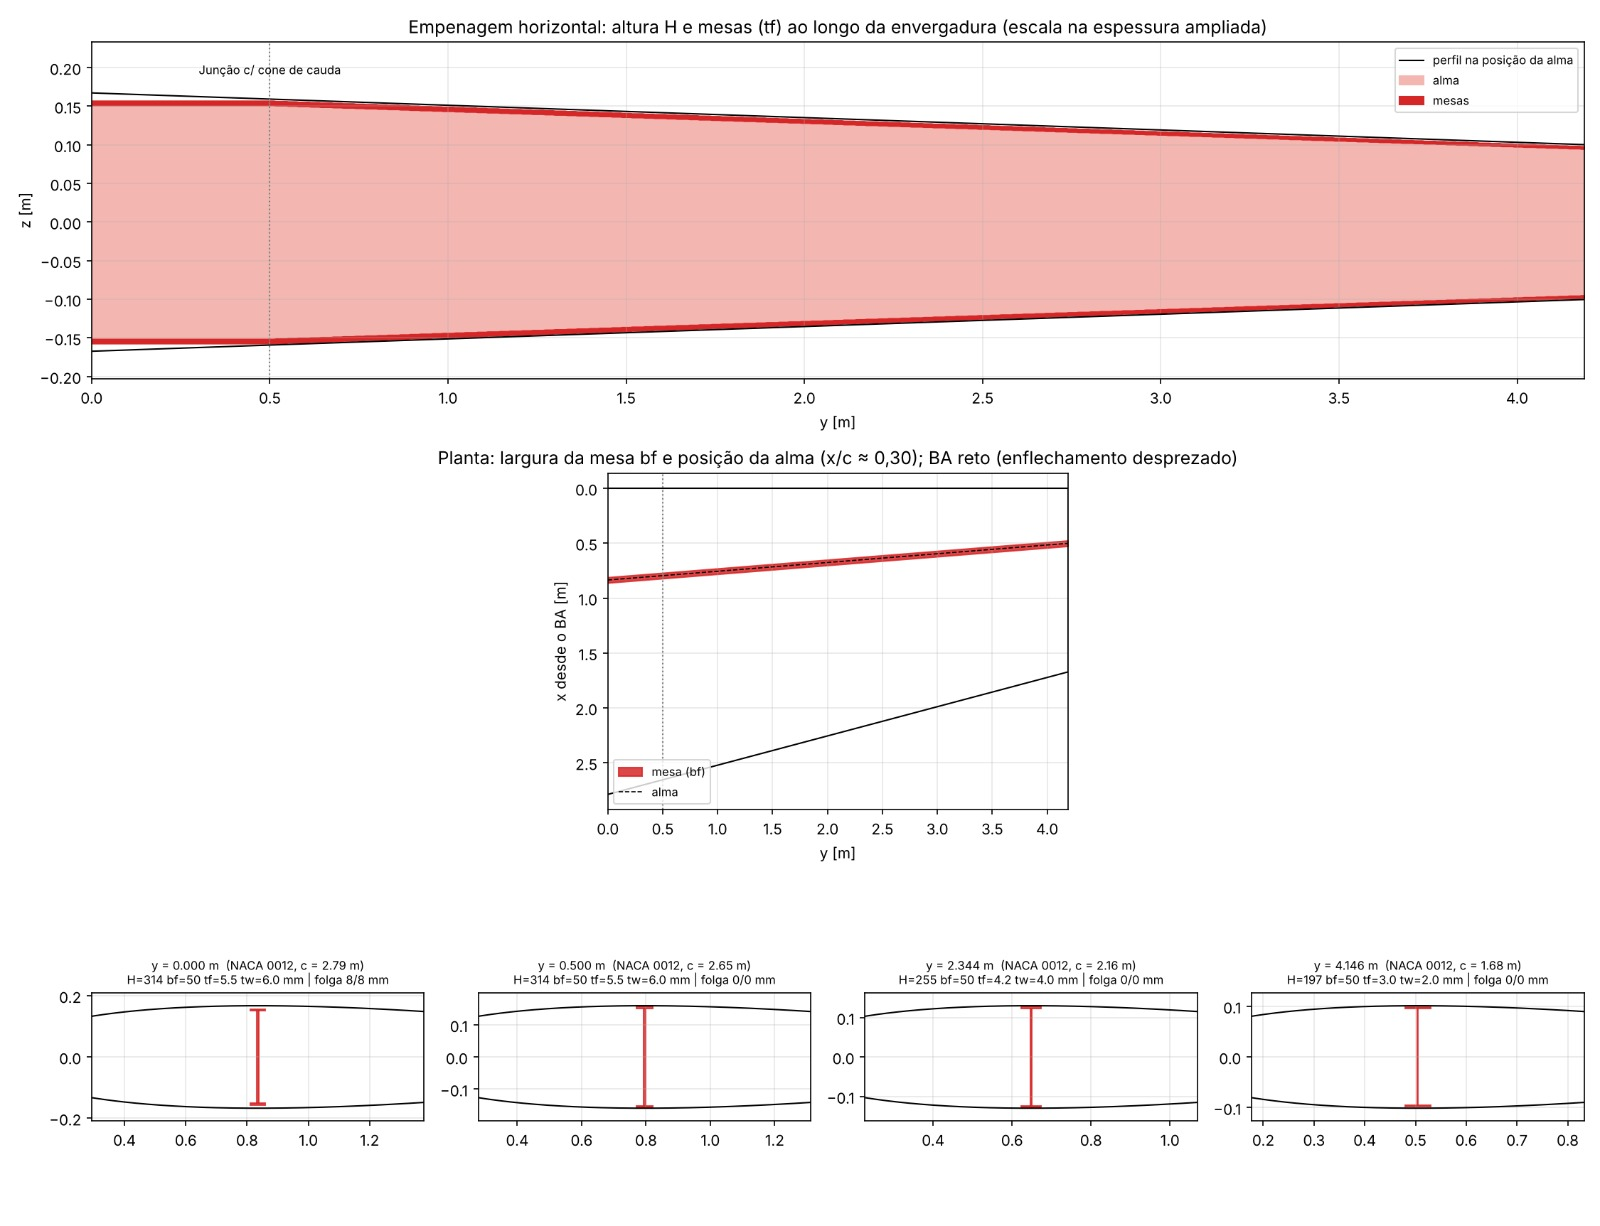
\includegraphics[width=1.0\textwidth]{eh_parte5_longarina.jpeg}
    \caption{Resumo do dimensionamento da longarina ao longo da semienvergadura: elevação (topo), vista em planta (centro) detalhando a posição da alma ($x_{alma}$), evolução geométrica da seção transversal e margens de segurança para os casos de carga críticos (fundo).}
    \label{fig:longarina_EH_resumo}
\end{figure}

\section{Empenagem Vertical}
\subsection{Longarina da EV}

O dimensionamento da longarina da empenagem vertical (EV) adota a mesma metodologia estrutural e os mesmos critérios de falha descritos para a seção da asa \ref{sec:secao_longarina_asa}. 

O material empregado permanece a liga de alumínio 7075-T6. A análise estrutural avalia os esforços atuantes decorrentes de dois casos de carga críticos específicos para a superfície vertical: LC63 e LC61.

A geometria da longarina apresenta uma seção transversal constante da base até a junção com a fuselagem, localizada na estação vertical $z = 0,335$ m. A partir desse ponto até a ponta da superfície, as dimensões da seção afilam linearmente, com a altura estrutural máxima limitada pela geometria do perfil aerodinâmico NACA 0012 local. A otimização geométrica do trecho constante resultou em uma seção com altura $H = 477$ mm, largura de mesa $b_f = 50$ mm, espessura de mesa $t_f = 3,5$ mm e espessura de alma $t_w = 7,0$ mm. Na estação da ponta, a seção atinge as dimensões mínimas de $H = 245$ mm, $b_f = 50$ mm, $t_f = 3,0$ mm e $t_w = 2,0$ mm, suficientes para manter as margens de segurança positivas. A massa estrutural total computada para a longarina completa da EV (uma única superfície) é de $29,4$ kg.

A tabela \ref{tab:longarina_ev_resultados} resume os valores das dimensões da longarina da EV em cada seção da mesma.

\begin{table}[H]
    \centering
    \caption{Distribuição das dimensões geométricas da longarina da EV e massa linear ao longo da altura.}
    \vspace{0.2cm}
    \begin{tabular}{cccccccc}
        \hline
        \textbf{$z$ [m]} & \textbf{Corda [m]} & \textbf{Perfil} & \textbf{$H$ [mm]} & \textbf{$b_f$ [mm]} & \textbf{$t_f$ [mm]} & \textbf{$t_w$ [mm]} & \textbf{Massa [kg/m]} \\
        \hline
        0,000 & 4,158 & NACA 0012 & 477 & 50,0 & 3,50 & 7,00 & 10,23 \\
        0,335 & 4,017 & NACA 0012 & 477 & 50,0 & 3,50 & 7,00 & 10,23 \\
        1,000 & 3,736 & NACA 0012 & 444 & 50,0 & 3,43 & 6,28 & 8,67 \\
        2,000 & 3,311 & NACA 0012 & 393 & 50,0 & 3,32 & 5,19 & 6,64 \\
        3,000 & 2,890 & NACA 0012 & 342 & 50,0 & 3,21 & 4,10 & 4,81 \\
        4,000 & 2,469 & NACA 0012 & 292 & 50,0 & 3,10 & 3,01 & 3,29 \\
        4,925 & 2,079 & NACA 0012 & 245 & 50,0 & 3,00 & 2,00 & 2,19 \\
        \hline
    \end{tabular}
    \label{tab:longarina_ev_resultados}
\end{table}

Na figura \ref{fig:longarina_EV_resumo}, são resumidas e apresentadas as dimensões da longarina ao longo da altura, bem como as margens de segurança e as folgas em algumas seções relevantes da EV.

\begin{figure}[H]
    \centering
    % Ajuste \textwidth para um tamanho menor se a imagem ficar grande demais
    % ou use \linewidth.
    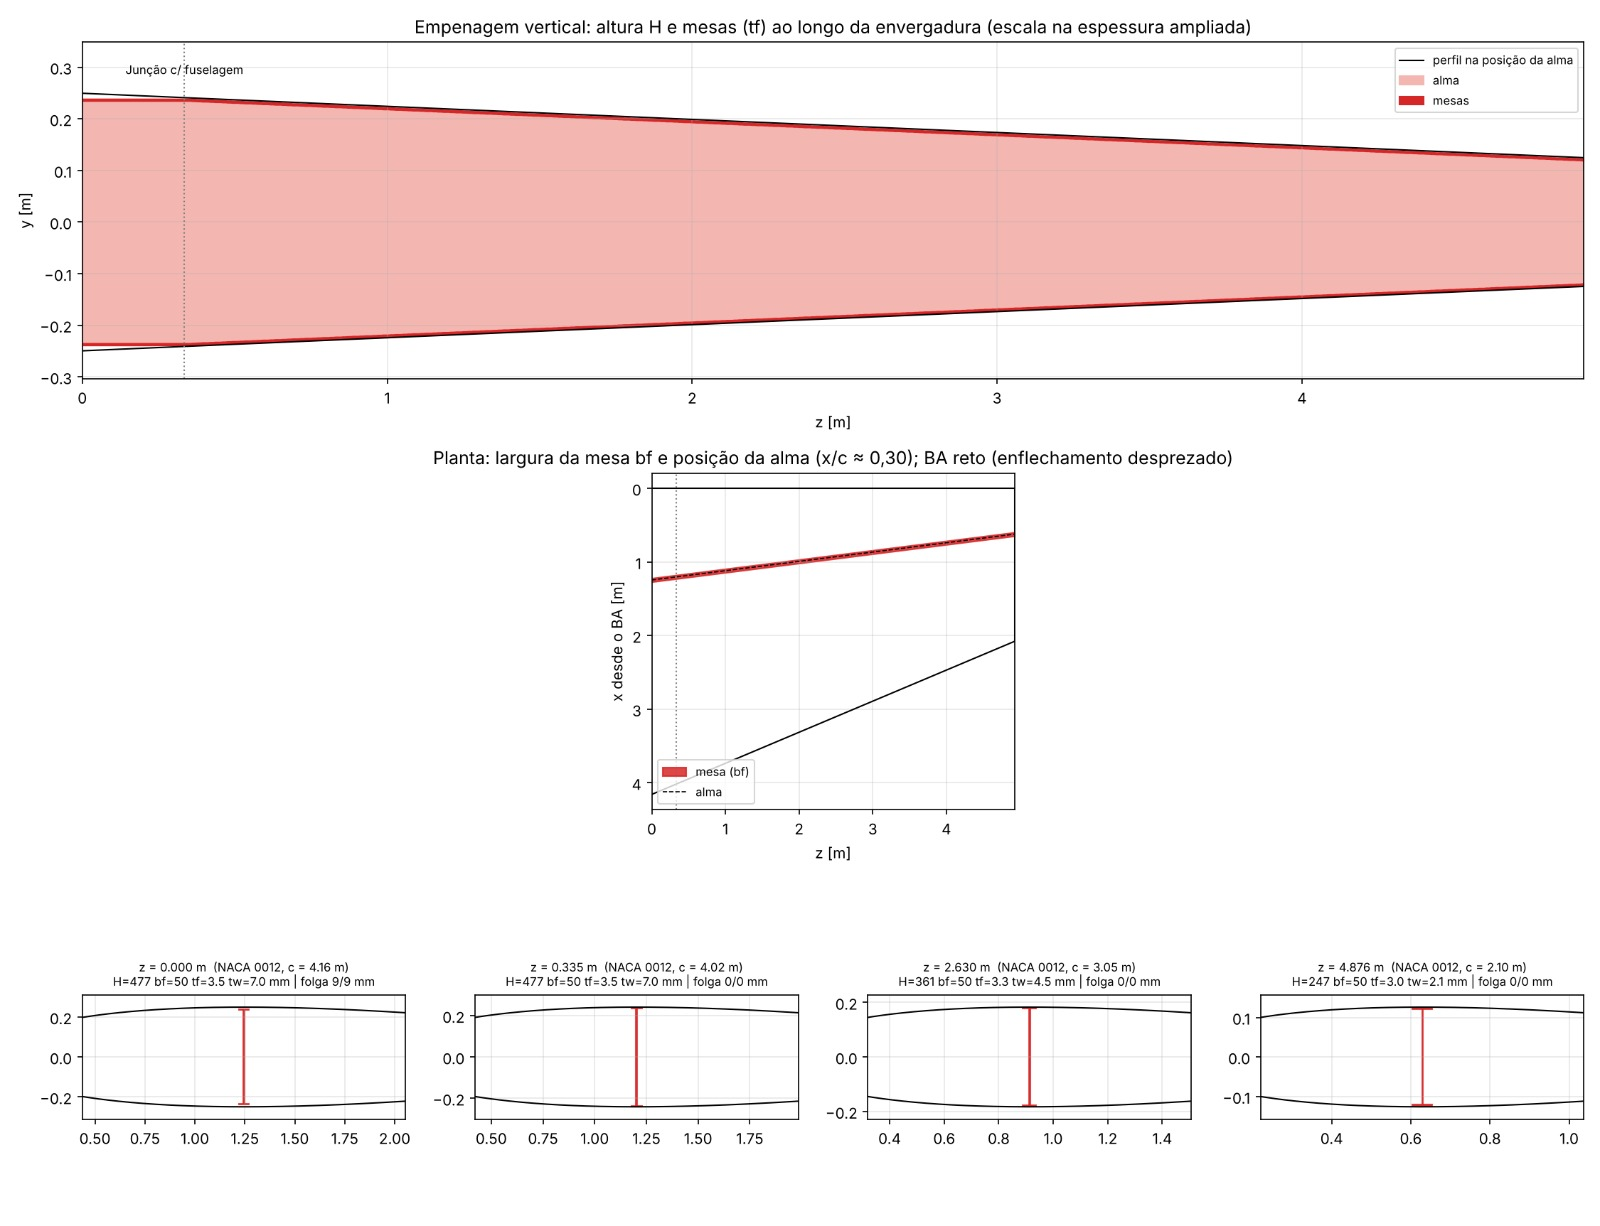
\includegraphics[width=1.0\textwidth]{ev_parte5_longarina.jpeg}
    \caption{Resumo do dimensionamento da longarina ao longo da altura da EV: elevação (topo), vista em planta (centro) detalhando a posição da alma ($x_{alma}$), evolução geométrica da seção transversal e margens de segurança para os casos de carga críticos (fundo).}
    \label{fig:longarina_EV_resumo}
\end{figure}

\section{Resumo das longarinas}

A tabela \ref{tab:resumo_longarinas} a seguir resume o dimensionamento das longarinas da Asa, da EH e da EV da aeronave, servindo como base para comparação entre elas e como cálculo preliminar do peso estrutural adicionado.

\begin{table}[H]
    \centering
    \caption{Resumo geral do dimensionamento das longarinas (Massa computada para a longarina inteira: asa e EH = duas metades, EV = uma).}
    \vspace{0.2cm}
    \resizebox{\textwidth}{!}{
    \begin{tabular}{lcccc}
        \hline
        \textbf{Superfície} & \textbf{Raiz: $H \times b_f \times t_f \times t_w$ [mm]} & \textbf{Ponta: $H \times b_f \times t_f \times t_w$ [mm]} & \textbf{Massa [kg]} & \textbf{MS mín (critério, caso)} \\
        \hline
        Asa & $402 \times 400 \times 33,0 \times 7,5$ & $120 \times 195 \times 3,0 \times 2,0$ & 1395,9 & $+0,006$ (resistência, LC4) \\
        Empenagem horizontal & $314 \times 50 \times 5,5 \times 6,0$ & $196 \times 50 \times 3,0 \times 2,0$ & 36,7 & $+0,038$ (resistência, LC10) \\
        Empenagem vertical & $477 \times 50 \times 3,5 \times 7,0$ & $245 \times 50 \times 3,0 \times 2,0$ & 29,4 & $+0,053$ (flambagem da alma, LC63) \\
        \hline
        \textbf{Total} & & & \textbf{1462,0} & \\
        \hline
    \end{tabular}
    }
    \label{tab:resumo_longarinas}
\end{table}

\begin{figure}[H]
    \centering
    \caption{Arranjo estrutural das empenagens.}
    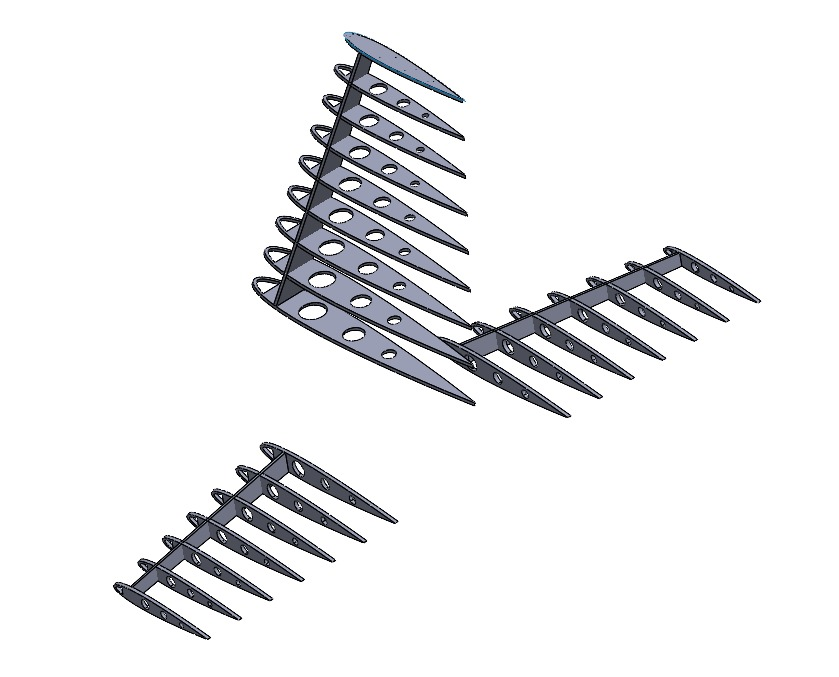
\includegraphics[width=0.6\textwidth]{Images-3-ProjetoDetalhado/cad-02.jpeg}
    \label{fig:cad_dimensionamento_2}
\end{figure}

\section{Fuselagem}
\label{sec:fuselagem}

A fuselagem foi dimensionada como uma casca semi-monocoque idealizada: cilindro de raio $R = 1{,}45$~m e comprimento $\ell = 16{,}0$~m, composta por revestimento, reforçadores longitudinais (\textit{stringers}) em Z e cavernas de seção retangular. A seção foi mantida constante.Adotou-se material único, liga Al 2024-T3 conforme propriedades da Tabela \ref{tab:propriedades_aluminio_si}.
 
A torção na fuselagem, constante entre a empenagem e a asa, foi tomada como o maior valor entre a contribuição da EV e a da EH:
\begin{equation}
  T_{EV} = M_{f,EV} + F_{EV}\, z_{EV}, \qquad
  T_{EH} = (1 - 0{,}8)\, M_{f,EH},
\end{equation}
com $M_{f}$ o fletor de raiz e $z_{EV}$ a altura da raiz da EV em relação ao eixo da fuselagem.
 
As condições consideradas são as críticas das empenagens: LC10 e LC41 (Tabela \ref{tab:cargas_criticas_eh}), e LC61 e LC63 (Tabela \ref{tab:cargas_criticas_ev}). As forças na direção $x$ das superfícies foram desprezadas por serem uma ordem de grandeza inferiores às forças em $z$ (EH) e em $y$ (EV).
 
O dimensionamento usa o envelope dos máximos ao longo do eixo longitudinal e entre condições, aplicados simultaneamente, o que é conservativo:
\begin{equation}
  M_u = FS\sqrt{M_{y,\max}^2 + M_{z,\max}^2}, \quad
  V_u = FS\sqrt{V_{z,\max}^2 + V_{y,\max}^2}, \quad
  T_u = FS \cdot T_{\max}, \qquad FS = 1{,}5 .
\end{equation}
% O trecho entre as longarinas foi excluído do envelope. Nesse trecho, o apoio em dois pontos produz um pico de cortante associado ao binário das reações, típico da região de transferência de carga, que pertence ao dimensionamento detalhado.
 
Como a massa da casca entra nas cargas de inércia, o cálculo é iterativo. Parte-se de uma estimativa de ($3000$~kg). Dimensiona-se, e a massa obtida realimenta as cargas até que a variação seja inferior a 1\%. A convergência ocorreu em 3 iterações.
 
\subsection{Critérios de dimensionamento}
 
As propriedades da seção usam a espessura equivalente $t_{eq} = t + A_s/b$ para tensões longitudinais, onde $A_s$ é a área de um reforçador e $b = 2\pi R/n_s$ o espaçamento entre reforçadores. Para cisalhamento e tensão circunferencial, considera-se apenas o revestimento. Na posição angular $\theta$ (medida a partir do ponto de flexão máxima):
\begin{equation}
  \sigma_x(\theta) = \frac{M_u}{\pi R^2 t_{eq}}\cos\theta + \frac{\Delta p_u R}{2\, t_{eq}}, \quad
  \sigma_\theta = \frac{\Delta p_u R}{t}, \quad
  \tau(\theta) = \frac{1}{t}\left(\frac{T_u}{2\pi R^2} + \frac{V_u}{\pi R}\sin\theta\right).
\end{equation}
 
Cada critério abaixo exige margem de segurança mínima $MS = F_{adm}/f - 1 \geq \pend{0{,}10}$, calculada na carga última.
 
\begin{enumerate}
  \item \textbf{Resistência do revestimento} (von Mises), varrendo $\theta \in [0,\pi]$, com e sem pressurização ($\Delta p_u = 1{,}5\,\Delta p$ e $\Delta p_u = 0$):
  \begin{equation}
    \sigma_{vm} = \sqrt{\sigma_x^2 - \sigma_x\sigma_\theta + \sigma_\theta^2 + 3\tau^2} \leq F_{tu}.
  \end{equation}
  \item \textbf{Pressão isolada} (FAR 25.365(d)): $1{,}33\,\Delta p$ como carga limite, com $\sigma_\theta \leq F_{ty}$ na limite e $\sigma_\theta \leq F_{tu}$ na última.
  \item \textbf{Compressão no reforçador}, sem pressurização: $\sigma_{st} = M_u/(\pi R^2 t_{eq}) \leq F_{cy}$.
  \item \textbf{Flambagem do painel} $b \times L$, sem pressurização, por interação compressão--cisalhamento de placa plana (a curvatura foi desprezada, o que é conservativo), com o revestimento sem flambar até $\pend{FS_{pan}}$ vezes a carga limite:
  \begin{equation}
    \begin{aligned}
      \sigma_{cr} &= k_c\frac{\pi^2 E}{12(1-\nu^2)}\left(\frac{t}{b}\right)^2, & \quad k_c &= \min_m\left(\frac{m b}{L} + \frac{L}{m b}\right)^2, \\[1ex]
      \tau_{cr} &= k_s\frac{\pi^2 E}{12(1-\nu^2)}\left(\frac{t}{b}\right)^2, & \quad k_s &= 5{,}35 + 4\left(\frac{b}{L}\right)^2,
    \end{aligned}
  \end{equation}
  \begin{equation}
    R_c + R_s^2 \leq 1, \qquad R_c = \sigma_c/\sigma_{cr}, \quad R_s = \tau/\tau_{cr},
  \end{equation}
  com $\sigma_{cr} \leq F_{cy}$ e $\tau_{cr} \leq F_{ty}/\sqrt{3}$ como cortes de plasticidade.
  
  \item \textbf{Coluna do reforçador} entre cavernas (reforçador mais a faixa de revestimento colaborante $b_e$), biapoiada, com comprimento efetivo $L$. Usa-se Euler para $L/\rho \geq \sqrt{2\pi^2E/F_{cy}}$ e Johnson caso contrário:
  \begin{equation}
    \sigma_{cr} = \frac{\pi^2 E}{(L/\rho)^2}
    \quad\text{ou}\quad
    \sigma_{cr} = F_{cy} - \frac{F_{cy}^2}{4\pi^2 E}\left(\frac{L}{\rho}\right)^2,
    \qquad \rho = \sqrt{I_{col}/A_{col}} .
  \end{equation}
  % O \textit{crippling} local foi substituído pela restrição geométrica $h_s/t_s \leq 30$, com flanges do Z iguais a $0{,}4\,h_s$.
  \item \textbf{Cavernas} pelo critério de rigidez de Shanley, para evitar instabilidade geral:
  \begin{equation}
    (EI)_{f} \geq (1 + MS)\, C_f\frac{M_u D^2}{L}, \qquad C_f = \frac{1}{16000}.
  \end{equation}
  Para a seção retangular $h \times w$, a massa por rigidez decresce com $h$, então a altura é definida pelas restrições adotadas: $h \leq \pend{100}$~mm, $h/w \leq 15$ e $w \geq \pend{1{,}5}$~mm.
\end{enumerate}
 
\subsection{Otimização}
 
O problema consiste em minimizar a massa da casca,
\begin{equation}
  m = \rho\,\ell\,\left(2\pi R\,t + n_s A_s\right) + n_f\,\rho\, h w\, 2\pi\!\left(R - \tfrac{h}{2}\right), \qquad n_f = \left\lfloor \ell/L \right\rfloor + 1,
\end{equation}
sujeito a todos os critérios da seção anterior. Foi feita uma busca exaustiva sobre um espaço discreto de projeto:
 
\begin{itemize}
  \item espessura do revestimento $t$: bitolas comerciais de 0,81 a 6,35~mm (15 valores);
  \item espessura do reforçador $t_s$: bitolas de 0,81 a 4,06~mm (10 valores);
  \item altura do reforçador $h_s$: 15 a 60~mm, espaçamento de 2,5~mm;
  \item número de reforçadores $n_s$: 40 a 240, múltiplos de 4, com espaçamento mínimo $b \geq \pend{100}$~mm (restrição de fabricação);
  \item espaçamento das cavernas $L$: 300 a 800~mm, espaçamento de 50~mm.
\end{itemize}
 
Para cada par $(L, n_s)$, todas as combinações $(t, t_s, h_s)$ são avaliadas simultaneamente. A caverna é dimensionada diretamente pelo critério de Shanley, pois depende apenas de $L$. A solução é a combinação viável de menor massa. Como o espaço é discreto e totalmente varrido, o mínimo obtido é global dentro do espaço considerado, sem dependência de ponto inicial. A verificação de que a solução não está na fronteira do espaço de busca confirma que o espaço foi suficiente. Esse laço de otimização fica dentro do laço de peso próprio.
 
\subsection{Resultados}
 
\begin{table}[H]
  \centering
  \caption{Esforços de envelope da fuselagem.}
  \begin{tabular}{lcc}
    \toprule
    Esforço & Limite & Último \\
    \midrule
    $M_{y,\max}$ ($x = 9{,}76$~m) [kN$\cdot$m] & 528,3 & -- \\
    $M_{z,\max}$ [kN$\cdot$m]                 & 293,1 & -- \\
    $M$ resultante [kN$\cdot$m]               & --    & 906,3 \\
    $V_{z,\max}$ / $V_{y,\max}$ [kN]          & 50,6 / 36,5 & -- \\
    $V$ resultante [kN]                       & --    & 93,6 \\
    $T_{\max}$ [kN$\cdot$m]                   & 108,1 & 162,2 \\
    \bottomrule
  \end{tabular}
\end{table}
 
As reações da asa sobre a fuselagem, obtidas por equilíbrio, foram de $-14{,}2$~kN (LC10) e $129{,}8$~kN (LC41).
 
\begin{table}[H]
  \centering
  \caption{Configuração de menor massa.}
  \begin{tabular}{llr}
    \toprule
    Componente & Parâmetro & Valor \\
    \midrule
    Revestimento      & espessura $t$ [mm]                   & 1,80 \\
    Reforçador & quantidade $n_s$ / espaçamento $b$ [mm]    & 88 / 103,5 \\
              & seção Z: $h_s \times t_s$, aba [mm]  & $22{,}5 \times 0{,}81$, 9,0 \\
              & área $A_s$ [mm$^2$]                  & 32,8 \\
              & esbeltez da coluna $L/\rho$          & 98,9 \\
    Cavernas  & espaçamento $L$ [mm] / quantidade    & 550 / 30 \\
              & seção retangular $h \times w$ [mm]   & $39{,}2 \times 2{,}62$ \\
              & $I$ / $I_{\text{Shanley}}$ [m$^4$]   & $1{,}316\times10^{-8}$ / $1{,}196\times10^{-8}$ \\
    \midrule
    Massa     & revestimento / reforçadores / cavernas [kg]     & \pend{729,2 / 128,4 / 77,0} \\
              & \textbf{total da casca} [kg]         & \textbf{934,7} \\
    \bottomrule
  \end{tabular}
\end{table}
 
A espessura do revestimento resultou governada pelos critérios de flexão e estabilidade, e não pela pressurização. A seção da caverna ficou limitada pela razão $h/w$ imposta, de modo que sua altura reflete essa restrição e não um ótimo estrutural. O reforçador resultou na menor bitola disponível ($t_s = 0{,}81$~mm), que corresponde ao limite inferior de fabricação adotado.
 
O envelope simultâneo de $M$, $V$ e $T$ e a seção constante tornam o resultado conservativo em massa. A seção constante obriga regiões menos solicitadas, como o nariz e cone de cauda, a usar a mesma seção da região crítica, junto à asa. Um zoneamento da espessura reduziria a massa.

A Figura \ref{fig:cad_dimensionamento_3} representa o arranjo estrutural final dos componentes críticos da aeronave.

\begin{figure}[H]
    \centering
    \caption{Arranjo estrutural da aeronave completa.}
    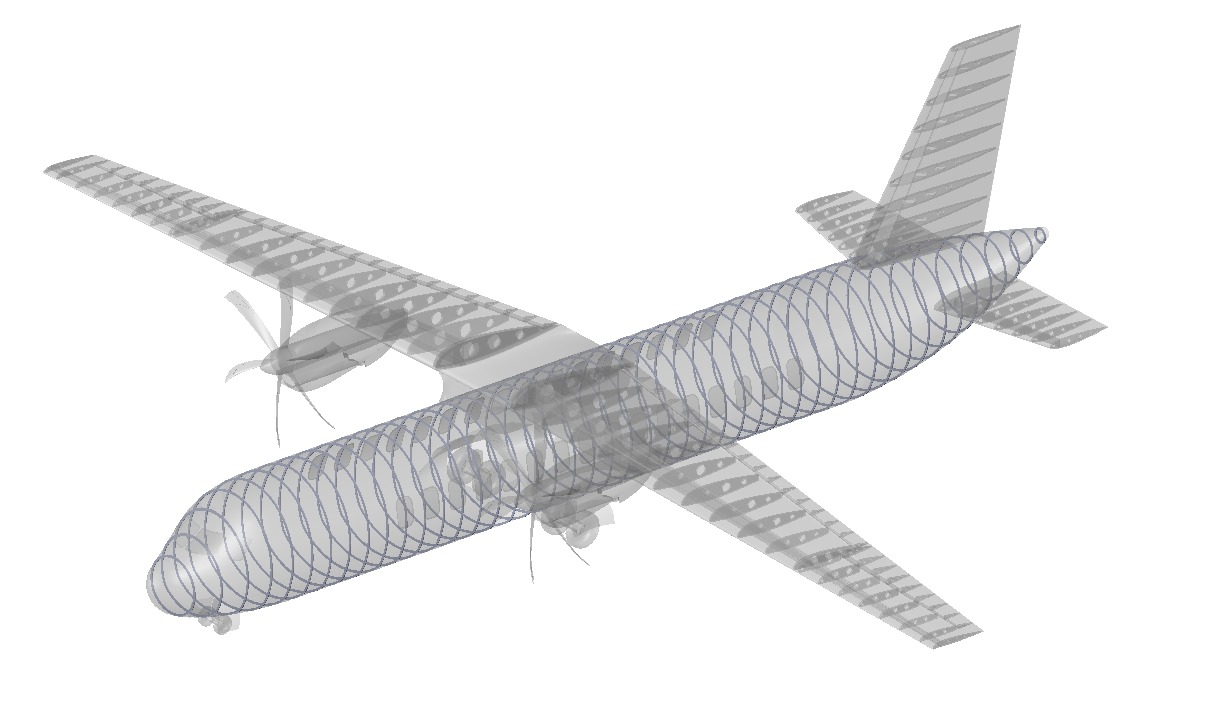
\includegraphics[width=1\textwidth]{Images-3-ProjetoDetalhado/cad-03.jpeg}
    \label{fig:cad_dimensionamento_3}
\end{figure}

